%% 
%% Copyright 2007-2020 Elsevier Ltd
%% 
%% This file is part of the 'Elsarticle Bundle'.
%% ---------------------------------------------
%% 
%% It may be distributed under the conditions of the LaTeX Project Public
%% License, either version 1.2 of this license or (at your option) any
%% later version.  The latest version of this license is in
%%    http://www.latex-project.org/lppl.txt
%% and version 1.2 or later is part of all distributions of LaTeX
%% version 1999/12/01 or later.
%% 
%% The list of all files belonging to the 'Elsarticle Bundle' is
%% given in the file `manifest.txt'.
%% 
%% Template article for Elsevier's document class `elsarticle'
%% with harvard style bibliographic references

%\documentclass[preprint,12pt,authoryear]{elsarticle}

%% Use the option review to obtain double line spacing
%% \documentclass[authoryear,preprint,review,12pt]{elsarticle}

%% Use the options 1p,twocolumn; 3p; 3p,twocolumn; 5p; or 5p,twocolumn
%% for a journal layout:
%% \documentclass[final,1p,times,authoryear]{elsarticle}
%% \documentclass[final,1p,times,twocolumn,authoryear]{elsarticle}
 \documentclass[final,3p,times,authoryear]{elsarticle}
%% \documentclass[final,3p,times,twocolumn,authoryear]{elsarticle}
%% \documentclass[final,5p,times,authoryear]{elsarticle}
%% \documentclass[final,5p,times,twocolumn,authoryear]{elsarticle}

%% For including figures, graphicx.sty has been loaded in
%% elsarticle.cls. If you prefer to use the old commands
%% please give \usepackage{epsfig}

%% The amssymb package provides various useful mathematical symbols
\usepackage{amssymb}
%% The amsthm package provides extended theorem environments
%% \usepackage{amsthm}

%% The lineno packages adds line numbers. Start line numbering with
%% \begin{linenumbers}, end it with \end{linenumbers}. Or switch it on
%% for the whole article with \linenumbers.
%% \usepackage{lineno}
%-----ADDED LATER---
\usepackage{mathtools,amssymb}
\usepackage[abs]{overpic}
\usepackage{xcolor,varwidth}
\usepackage{tikz}
\newcommand*\circled[1]{\tikz[baseline=(char.base)]{
		\node[shape=circle,draw,inner sep=1pt] (char) {#1};}}

%\usepackage{setspace}
%\setstretch{1.6}
%\usepackage[status=draft,layout=margin]{fixme}


%% The lineno packages adds line numbers. Start line numbering with
%% \begin{linenumbers}, end it with \end{linenumbers}. Or switch it on
%% for the whole article with \linenumbers.
%% \usepackage{lineno}

\journal{Journal of Fluids and Structures}

\begin{document}
	
	\begin{frontmatter}
		\title{Generating periodic vortex pairs using flexible structures}
		
		\author[inst1]{Gaurav Singh}
		\affiliation[inst1]{organization={Advanced Technology and Development Centre},
			addressline={Indian Institute of Technology Kharagpur}, 
			city={West Midnapore},
			postcode={721302}, 
			state={W.B.},
			country={India}}
		
		\author[inst1,inst3]{Arnab Atta}
		\author[inst1,inst2]{Rajaram Lakkaraju}
		
		\affiliation[inst2]{organization={Department of Mechanical Engineering},
			addressline={Indian Institute of Technology Kharagpur}, 
			city={West Midnapore},
			postcode={721302}, 
			state={W.B.},
			country={India}}
		
		\affiliation[inst3]{organization={Department of Chemical Engineering},
			addressline={Indian Institute of Technology Kharagpur}, 
			city={West Midnapore},
			postcode={721302}, 
			state={W.B.},
			country={India}}
		
		%The understanding of the vortex formation process is currently driving a novel attempt to evaluate the performance of fluid dynamics in biological systems. The concept of formation time, developed for axially symmetric orifices, is here studied in two- dimensional flows for the generation of vortex pairs. The early stage of the formation process is studied with the single vortex model in the inviscid limit. Within this framework, the equation can be written in a universal form in terms of the formation time. The single vortex model properly represents the initial circular spiralling vortex sheet and its acceleration for self-induced motion. Then, an analysis is performed by numerical simulation of the two-dimensional Navier–Stokes equations to cope with the spatially extended vortex structure. The results do not show the pinch- off phenomenon previously reported for vortex rings. The two-dimensional vortex pair tends to a stably growing structure such that, while it translates and extends longitudinally, it remains connected to the sharp edge by a shear layer whose velocity is always about twice that of the leading vortex. At larger values of the Reynolds number the instability of the shear layer develops small-scale vortices capable of destabilizing the coherent vortex growth. The absence of a critical formation number for two-dimensional vortex pairs suggests further considerations for the development of concepts of optimal vortex formation from orifices with variable curvature or of a tapered shape.
		
		\begin{abstract}
			In fluid dynamics, the starting flow through a narrow slit gives rise to a distinctive fluid mass due to the lateral rolling caused by vorticity induced at the slit tip. This process generates a counter-rotating vortex pair in planar or two-dimensional flows. In this study, considering a flow evolution model, we show that the growth rate of this ejected fluid rate scales as $\propto \sqrt{time}$. We draw a comparison on how does this vortex pair behave in an in-channel doamin which has bounded the wall boundaries. We observed that bounded walls amplify vorticity, and lower the leading vortex pair's progression rate due to the wall offered resistance. In contrast, the bounded channel walls sustain the vortex pair's form for an extended duration before they diffuse away as shear layer instabilities take effect. It is known that these vortex pairs do not undergo any propulsive detachment known as `pinch-off' from the tip-attached fluid layer. This study envision to instigate 'pinch-off' phenomenon in these vortex pairs using flexible slit walls, aiming to enhance the momentum transport potential of vortex pairs capitalizing on their self-propagating properties.
			Transitioning our focus to flexible slit walls, we unveil that the mutual relationship between flexible structures and fluid dynamics holds significance in diverse applications such as vortex formation and flow modulation. The flexibility of these plates prompts them to adapt under fluid forces and exhibit temporally oscillating behavior of the slit gap. We unearth a critical plate flexibility case which induces pinch-off in the resultant vortex pair, a phenomenon absent in the case of rigid plates. We explain that this pinch-off phenomenon is associated with the time scale of the oscillatory retraction of the flexible plates. The induced periodic pinch-off in the flow subsequently forms a train of vortex pairs through the channel. Furthermore, the study highlights the maximum propagation rate of the leading vortex pair in the channel, observed at a specific plate flexibility case with critical Cauchy number $=0.04$. These findings contribute to an enhanced understanding of fluid-structure dynamics, with broader implications in engineering and physics. The newfound insights into inducing and controlling vortex pair behaviors pave the way for innovative applications in various domains, spanning from fluid transport to advanced flow manipulation techniques.
			
		
		\end{abstract}
	
	
	

%		\begin{abstract}
%			A flow passing through a narrow slit results out in the form of a fluid mass because of the lateral roll-up caused by slit tip induced vorticity. The ejected mass flow in a two-dimensional flow consists of a counter rotating vortex pair. It is known that such vortex pairs evolve over time but do not get pinched-off (a propulsive detachment phenomenon) from the tip attached fluid layer. In this work, we aim to trigger the pinch off in such vortex pairs by employing flexible slit walls. This pinch-off of vortex pairs shall help in momentum transport to a longer distance due to their self-propagating property. We begin the study by comparing the formation and growth of vortex pairs in a bounded in-channel flow domain and its comparison with unbounded wide system. The wall boundaries induce larger vorticity as the flow grows and henceforth, the resistance reduces the propagation rate of the leading vortex pair. The bounded channel, however, ensures the vortex pair to ensure its form for a longer time before the shear layer instabilities kick-in. We then investigate the role of flexible plates' as slit walls. Understanding the interplay between flexible structures and fluid dynamics is pivotal in numerous applications, including vortex formation and flow control. As fluid flows over these plates, the inherent plates' flexibility causes them to morph in response to fluid forces. The study investigates the slit gap's temporal behavior, quantifying its oscillatory nature for various plate flexibility levels. This analysis exposes a non-linear relationship between plate flexibility and the gap width, akin to different slit gap sizes. We find that at a critical plates' flexibility case, the pinch-off of the resulting vortex pair is observed which was absent in rigid place case. The frequency of pinched-off vortices is found to be associated with the time-scale of back motion of the flexible plates' oscillation. In addition to that the imprint of periodic ejection in the form a train of vortex pair.  Additionally, We also found that the leading vortex pair propagates in the channel achieves a maxima for Cauchy number $= 0.04$ case. These results advances our comprehension of fluid-structure dynamics and their broader applications in engineering and physics.
%		\end{abstract}

%		\begin{abstract}
%			We present an in-depth analysis of the interaction between steady fluid flow through a narrow opening formed by two flexible plates, and the subsequent periodicity in the outflow prompted by the fluttering of the plates. Our exploration delineates the correlation between the oscillatory behaviour of the plates and the pulsatile nature of the subsequent fluid outflow, while concurrently scrutinizing the mechanics underpinning this interaction. We have investigated the 
%			
%			We unveil that the shear layer, initiated by the oscillation of the flexible plates, triggers the Kelvin-Helmholtz instability, leading to the creation of a vortex pair which subsequently advects into the subsequent downstream channel.
%			
%			
%		\end{abstract}


	\end{frontmatter}

%	\newpage

	\section{Introduction}
	\label{sec:Introduction}
	
	%-One particular aspect of vortex dynamics that has received significant attention is the formation and growth of vortex pairs. A vortex pair, typically arising from the roll-up of a shear layer, plays a critical role in various fluidic phenomena such as the start-up flow in a channel, wake generation behind an object, and many others. The focus of this research is to delve into the mechanics of the vortex pair, specifically the Leading Vortex Pair (LVP), within a narrow slit environment and to understand the implications of flexible versus rigid plates on its formation, propagation, and growth. 
	
	
	Throughout the annals of natural and scientific observation, one can identify instances of periodic vortex pairs or 'vortex dipoles' across various domains. These pairs are a marvel of physics, typically consisting of two oppositely rotating vortices of equivalent strength. Their prevalence can be noted in diverse natural processes such as animal locomotion, heart flow, and geophysical dipolar vortical structures found in large bodies of water \citep{Costello2002, gharib2005,mohseni_2015, salsac_2006, Kheradvar2010, gopalakrishnan_2014, Ahlnas1987, Borve_2021}. A vortex pair comes into existence when a fluid is impulsively thrust through a sudden opening in a channel, a process that is constrained by the sharp edges of the opening. This thrust causes the flow to separate and subsequently form two free shear layers at each edge. In turn, these layers curl up into a spiral, resulting in a vortex pair \citep{Blondeaux1983}. These two vortices are initially tied together by a local dependence on flow over a sharp edge, which can be understood through the lens of similarity law \cite{Rott1956, Pullin1978}. However, as this local dependence dissolves, the spiralled-up vortex structure becomes influenced by the overarching flow \citep{Pullin1978, pullin_perry_1980}.
	
	Upon their formation, these vortices possess self-induced velocity and, even with the reduction of the inlet flow, they can continue their downstream propagation, thus demonstrating a net linear momentum \citep{Barker1977}. Consequently, vortex pairs become crucial agents in the transport of mass and heat within a flow due to their self-propagating nature. An interesting manifestation of this transport mechanism can be observed in the oceanic ecosystem where vortex pairs can ensnare passive scalars such as phytoplanktons within their cores, facilitating their transport over vast distances \citep{Provenzale1999}. This aspect makes the study of the generation of vortex pairs of paramount importance to our understanding of momentum transport systems. During the evolutionary journey of a vortex pair through a constriction, an interesting phenomenon emerges where the vortex structure manages to acquire a saturated circulation and a velocity higher than the attached shear layer, all without disengaging from the shear layer at the exit. This process, known as 'pinch-off', has been extensively observed in an axisymmetric three-dimensional (3D) counterpart of a vortex pair, referred to as a 'vortex ring' \citep{Gharib1998}.
	
	However, the behaviour of a two-dimensional (2D) vortex pair diverges from its 3D counterpart in a key aspect: a 2D vortex pair continues to grow as long as it receives sustenance from the inlet source. This concept was put to test in a landmark experiment by \cite{Afanasyev2006}, where a layered fluid system (comprising two fluids with distinct densities) was used to facilitate a 2D flow at Reynolds number, $Re \approx\mathcal{O}(100)$. Notably, the emerging vortex pair did not demonstrate any vortex stretching or an increase in enstrophy, and the pinch-off was conspicuously absent. In a quasi-2D experimental setup, \cite{domenichini_2011} corroborated this absence of pinch-off while observing vortex loop formation through a slender opening past two semi-circular ends. Further evidence for the discrepancy in 2D and 3D vortex structures was provided by \cite{ofarrell_dabiri_2012}, who suggested that a 2D vortex pair achieves a lower translational velocity and larger streamwise expansion, thereby promoting a continuous growth without any disruption. Another notable finding was presented by \cite{pedrizzetti_2010} that showcased the vortex pair's stability in growth as it elongates longitudinally while still connected to the trailing shear layer. Nonetheless, the stability of the vortex pair faces a significant challenge when the Reynolds number, $Re$, crosses a critical threshold (approximately 5000). At such high $Re$ values, the attached vorticity layers become unstable, causing smaller vortices to roll up behind the detached pair. The emergent smaller vortical structures disrupt the coherence of the leading vortex pair, eventually breaking away \citep{luchini_tognaccini_2002}. This detachment phenomenon, although reminiscent of the 'pinch-off' observed in 3D vortex rings, differs fundamentally in its causation. Unlike pinch-off, the detachment in high $Re$ vortex pairs is triggered by the instability and resulting incoherence of the shear layers. As such, no isolated, compact vortex pair can be identified in these circumstances. 
	
	Furthermore, the velocity of the detached pair is significantly lower than that of the trailing shear layer, causing the vortex pair to spread laterally rather than traveling longer streamwise distances. The initiation of this instability, which marks the detachment of the vortex pair, necessitates the introduction of a new characteristic time-scale called 'start-up time', as first introduced by \cite{Afanasyev2006}. In Afanasyev's experiments, conducted at $Re\approx \mathcal{O}100$, the start-up time was found to be 15. Another significant contribution came from \cite{pedrizzetti_2010}, who showed that a vortex pair can grow stably at $Re\approx2000$ up to the start-up time of 10. Similarly, \cite{Gao_Yu_2016} found that the separation of the leading vortex pair occurred at the start-up time of 7 for the experiments conducted at $Re\approx1500-3400$. Thus, it becomes clear that the start-up time, marking the onset of shear layer instability, is indeed a manifestation of the flow transition, which is hastened by an increase in $Re$. However, if we are to optimize the generation of 2D vortex pairs as an efficient momentum transport system, the question arises: how can we induce the 'pinch-off' phenomenon in a 2D vortex pair formation process? The answer, as suggested by this work, is to introduce a passive perturbation into the evolution process of the rolled-up shear layers.
	\begin{figure}[h]
		\centering
		\begin{minipage}[c]{0.95\linewidth}
			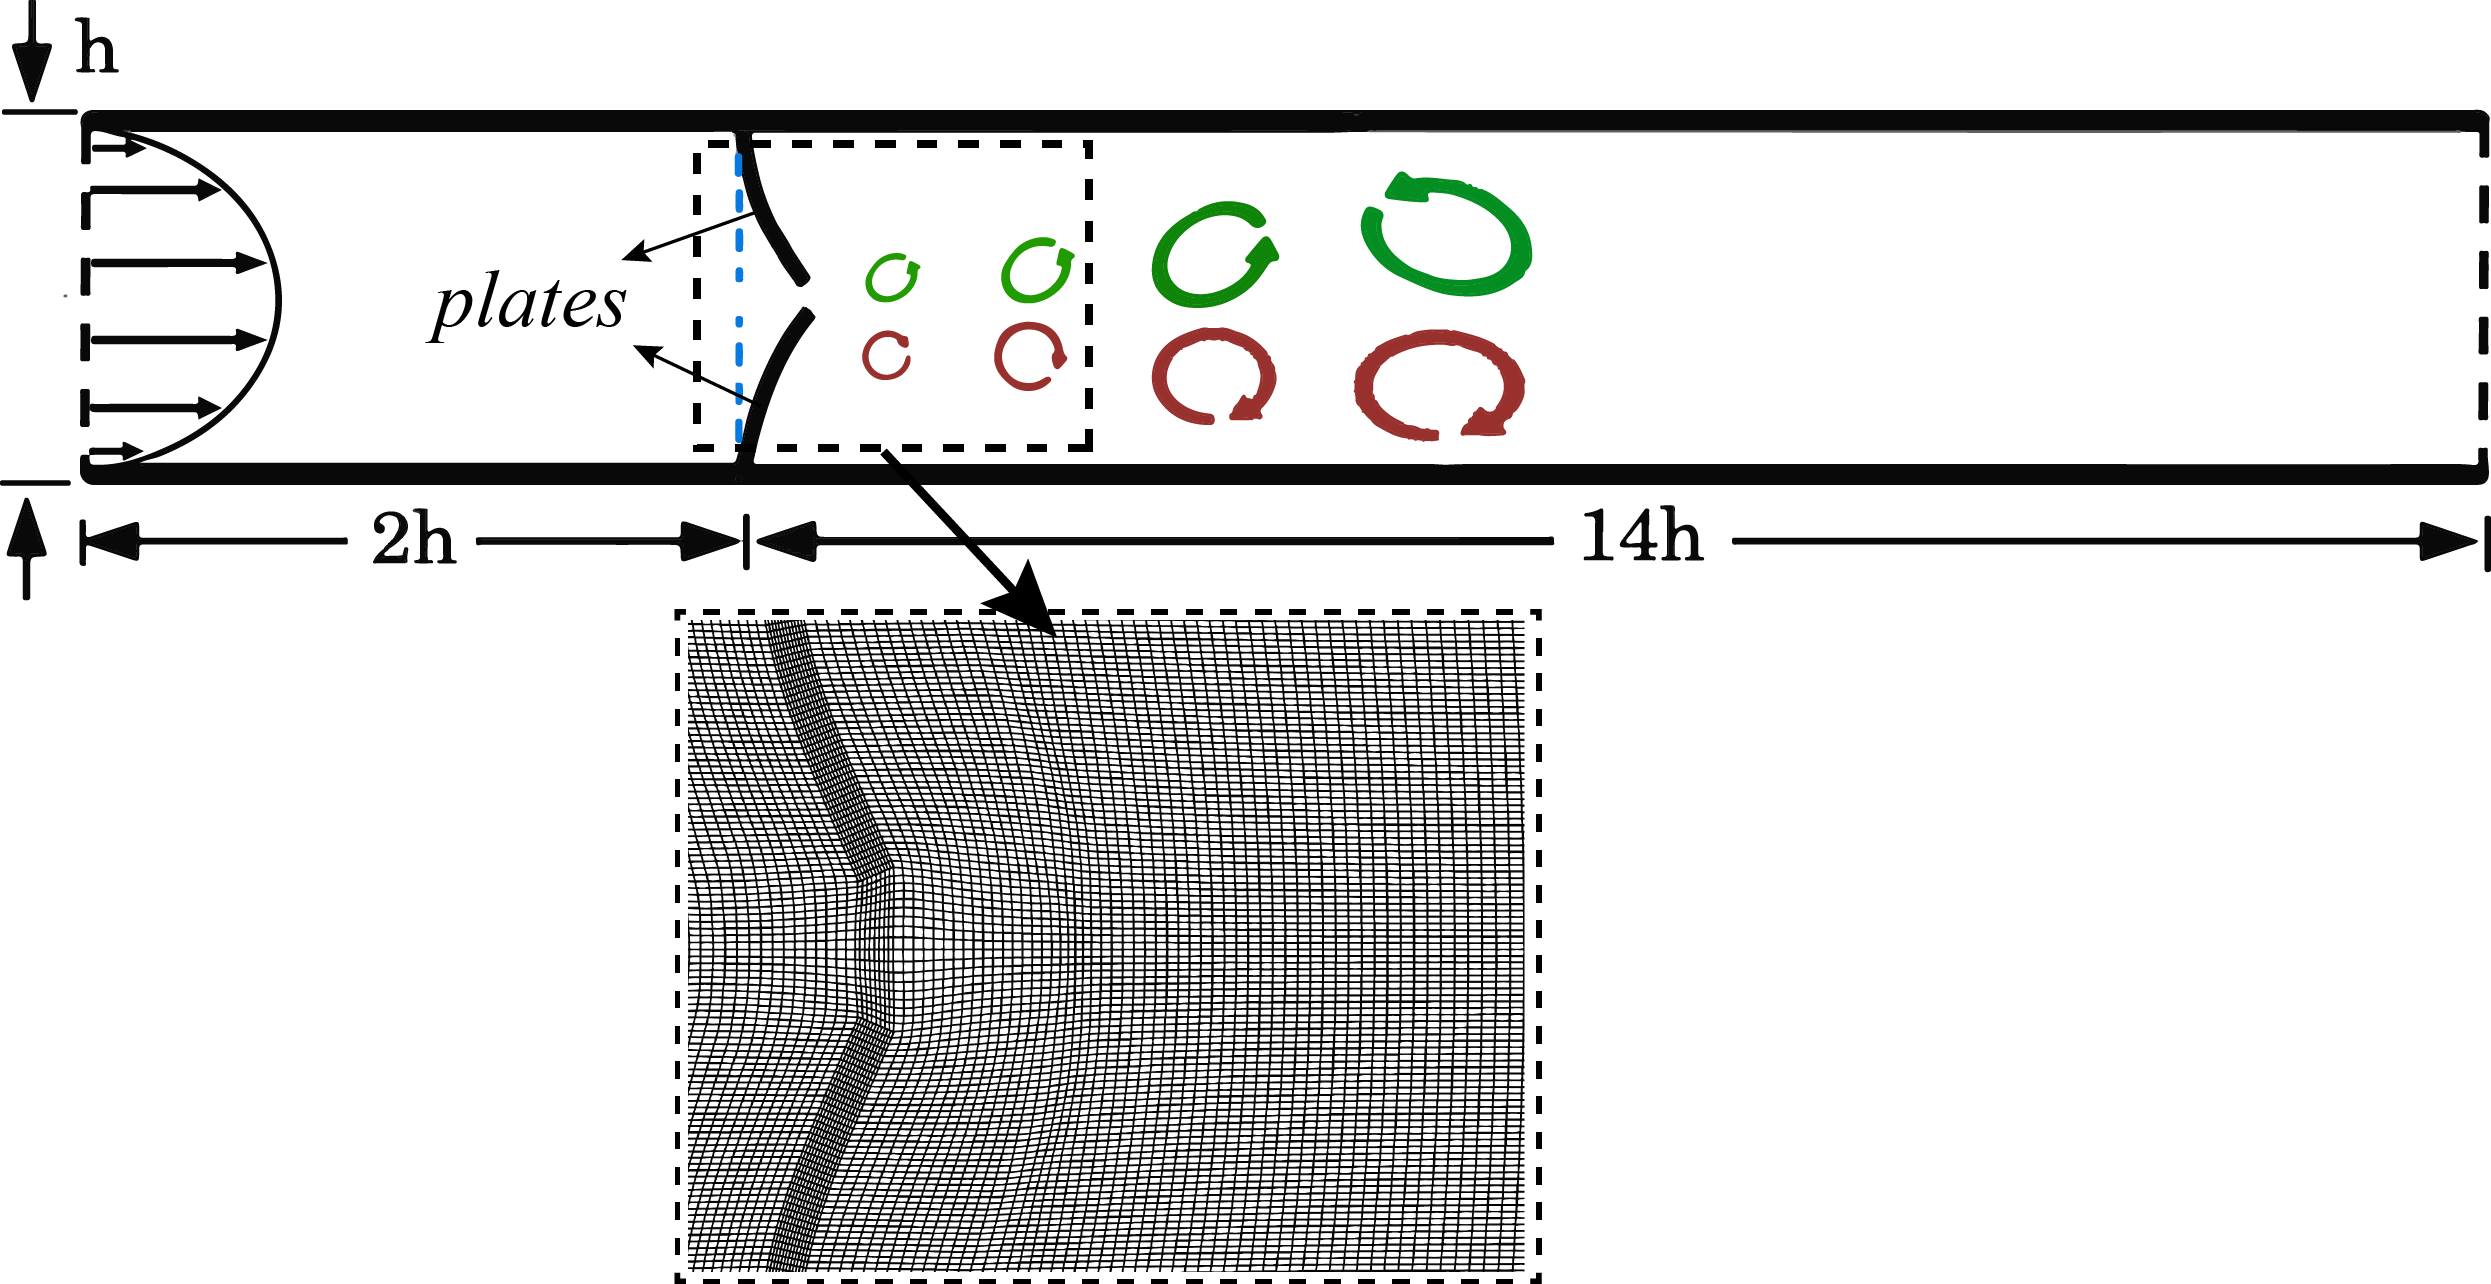
\includegraphics[width=1\linewidth]{Figures/Schematic-01.png} 
		\end{minipage} 		
		\caption{Schematic of the fluid flow past wall-mounted flexible plates in a channel. A fully developed flow enters from the inlet (left), passes through the slit between the two oppositely mounted plates, and leaves the channel from the outlet (right). Due to the flexibility of the mounted plates, the slit gap varies under the effect of inlet flow and causes vortical flow structures in the downstream domain. A typical mesh grid used is shown for the near-plate section of the channel featuring dynamic mesh motion.}	
		\label{fig:schematic}
	\end{figure}

	In this context, it is worthwhile to recall the experiment by \cite{arakeri_2013} where a piston-cylinder mechanism was employed to generate a starting jet. This jet emanated out of a channel exit equipped with two rigid flaps hinged parallel to the exit. Measurements showed that these hinged flap motions could significantly alter the flow, leading to the generation of two additional vortex pairs (compared to the rigid exit case) in one flow cycle. Building upon this work, \cite{arakeri_2018} replaced the hinged flaps with two flexible ones in the same setup. As the flow passed through the exit, the flexible flaps exhibited deformation due to the variation in pressure in the area, opening and closing accordingly. This two-way force exchange between the fluid and the structure brought about substantial changes to the outgoing flow and redistributed the vorticity structure, resulting in the creation of four vortex structures in one flow cycle due to the flap motion. These experiments were successful in perturbing the flow and redistributing the vorticity field using movable structures within the geometry. Nevertheless, the studies were primarily concerned with delivering higher impulse to the vortex pair generating setup. The vortex pairs that were ejected in these experiments did not venture downstream; instead, they spread laterally around the exit.
	
	Pursuing similar paths to induce vorticity redistribution, we present our study wherein we pass starting two dimensional flow past flexible plates mounted on opposite channel walls, replacing the rigid exit. The incoming flow strikes these plates normally, exits through the gap between the two plates, and evolves into a vortex pair. This study further explores the role of the plates' flexural rigidity and its effects on subsequent flow to potentially cause pinch-off and generate isolated vortex pairs. A detailed discussion of the impact of the slit gap's adaptability (static or dynamic) on the propagation and pinch-off of the vortex pairs will be presented. 
	
 %The complexity of the vortex motion, especially within a confined system, presents numerous challenges in understanding and predicting their formation, behavior, and subsequent implications.



\begin{figure}[h]
	\centering
	\begin{minipage}[c]{0.77\linewidth}
		\begin{overpic}[width=0.97\linewidth,height=1.5cm,trim=100 0 600 0, clip]{Figures/Figures/Jet/1S/1S_0100.png}
			\put(-25,20){{\parbox{0.4\linewidth}{$(a)$}}}
			\put(70,20){{\parbox{0.4\linewidth}{$LVP$}}}
		\end{overpic}
		%	\tikz \draw (0,0) ellipse (2cm and 1cm)
		\begin{overpic}[width=0.97\linewidth,height=1.5cm,trim=100 0 600 0, clip]{Figures/Figures/Jet/1S/1S_0500.png}
			\put(-25,20){{\parbox{0.4\linewidth}{$(b)$}}}
		\end{overpic}
		\begin{overpic}[width=0.97\linewidth,height=1.5cm,trim=100 0 600 0, clip]{Figures/Figures/Jet/1S/1S_0950.png}
			\put(-25,20){{\parbox{0.4\linewidth}{$(c)$}}}
			\put(60,27){{\parbox{0.4\linewidth}{$trailing \ shear \ layer$}}}
		\end{overpic}
		\begin{overpic}[width=0.97\linewidth,height=1.5cm,trim=100 0 600 0, clip]{Figures/Figures/Jet/1S/1S_1400.png}
			\put(-25,20){{\parbox{0.4\linewidth}{$(d)$}}}
			\put(160,8){{\parbox{0.4\linewidth}{$detachment$}}}
		\end{overpic}		
		%		\begin{overpic}[width=0.97\linewidth,height=1.5cm,trim=100 0 600 0, clip]{Figures/Figures/Jet/1S/1S_1850.png}
			%			\put(-25,20){{\parbox{0.4\linewidth}{$(e)$}}}
			%		\end{overpic}
	\end{minipage}
	\begin{minipage}[c]{0.03\linewidth}
		\centering
		\begin{overpic}[width=0.75\linewidth,height= 3.5cm]{Figures/Figures/Jet/1S/leg3.png}
			\put(14,52){{\parbox{0.4\linewidth}{\rotatebox{90}{\Large$u_x/u_o$}}}}
			\put(14,95){{\parbox{0.4\linewidth}{\Large$8$}}}
			\put(14,2){{\parbox{0.4\linewidth}{\Large$1$}}}		
		\end{overpic}
	\end{minipage} 
	\caption{Contour of instantaneous stream-wise velocity of the flow through slit between the rigid plates normalised by the inlet flow velocity $u_x/u_0$. Time snapshots are at instances $t/\tau \approx 7,\ 35,\ 70,\ 103 $ for each panel respectively.}
	\label{fig:Ux_contour_1S}
\end{figure}
	\section{Methods}\label{sec:maths}
	\subsection{Governing equations and the numerical method}\label{subsec:maths}
	We have performed numerical simulations of the discussed in the schematic problem. The simulations consist of interaction between the plates and the fluid coupled strongly so as to exchange forces in both ways. The finite volume method of numerical simulations is performed without any turbulence models. the plates' motion is a result of the dynamic interaction between incoming flow and the plates' feedback. The governing equations for the flow are the two-dimensional, incompressible, unsteady Navier-Stokes equations which read as
	\begin{eqnarray}
		\nabla\cdot\left[(\mathbf{u}_f-\mathbf{u}_m)\right] &=& 0, \\
		\rho_f\left[{\partial\mathbf{u}_f\over\partial t}+\left[(\mathbf{u}_f-\mathbf{u}_m)\cdot\mathbf{\nabla}\right]\mathbf{u}_f\right] &=& \mathbf{\nabla}\cdot\mathbf{\boldsymbol{\sigma}}_f,
	\end{eqnarray}
	
	where $\mathbf{u}_f=(u_x,u_y)$ is the velocity of the flow, $\mathbf{u_m}$ is the mesh motion velocity, $\rho_f$ is the fluid density, and $\boldsymbol{\sigma}_f$ is the total stress tensor in the fluid. Here, $\mathbf{\nabla}\equiv ({\partial\over\partial x},{\partial\over\partial y})$ is the spatial gradient for two-dimensions (x-y plane) and ${\partial\over\partial t}$ is the partial derivative operator with time.	Divergence of the stress tensor read as $\nabla\cdot\boldsymbol{\sigma}_f=-\mathbf{\nabla}P+\mu_f\mathbf{\nabla}^2\mathbf{u}_f$ for the incompressible and Newtonian fluid, where $P$ is dynamic pressure, $\mu_f$ is the fluid dynamic viscosity and $\nabla^2$ is laplacian operator. We have considered the strong coupling methodology between the fluid and the plate (structure) so as to accommodate two-way mutual interaction as discussed before. The governing equations for such couplings are formulated by using the Arbitrary Lagrangian Eulerian (ALE) framework, in which the volume change of each grid element between two subsequent time steps is always equal to the volume swept by the mesh, see more details in~\citep{Nguyen2010, Slone2002, CampbellPaterson2011}.  %The plates' motion (or the displacement, $\mathbf{u}_s$), is computed on the Arbitrary Lagrangian framework on which the mesh velocity ($\mathbf{u}_m$) equals the material velocity, i.e., $\mathbf{u}_m\equiv {\partial\mathbf{u}_s\over\partial t}$. The Eulerian mesh (for the fluid) implementation follows $\mathbf{u}_m=0$, and for the Lagrangian mesh, it follows $\mathbf{u}_m=\mathbf{u}_f$.
	The governing equation considered for the flexible plate is given by,	
	\begin{eqnarray}
		\rho_s{\partial^2\mathbf{u}_s\over\partial t^2} &=& \mathbf{\nabla}\cdot\mathbf{\boldsymbol{\sigma}}_s,
	\end{eqnarray}
	where $\rho_s$ is the density of the plate, $\mathbf{u}_s$ is the plates' motion velocity, and $\mathbf{\boldsymbol{\sigma}}_s$ is the Cauchy stress tensor. We have assumed a linear elastic material property for the plate, in which the strain rate is defined as per Lagrangian-Green's tensor, $\boldsymbol{\varepsilon}_s={1\over2}(\mathbf{\nabla}\mathbf{u}_s+\mathbf{\nabla}\mathbf{u}_s^T+\mathbf{\nabla}\mathbf{u}_s^T \cdot \mathbf{\nabla}\mathbf{u}_s)$. The stress and strain tensors are constituted as $\boldsymbol{\sigma}_s=2\mu_s \boldsymbol{\varepsilon}_s+\lambda( \mathbf{\nabla}\cdot\mathbf{u}_s)\mathcal{I}$, where $\mu_s=\mathcal{E}/[2(1+\kappa)]$ and $\lambda=\kappa \mathcal{E}/[(1+\kappa)(1-2\kappa)]$ are the Lame's constants, $\mathcal{E}$ is the Young's modulus, $\kappa$ is the Poisson's ratio,  and $\mathcal{I}$ is a rank two identity tensor. The superscript $^T$ here represents transpose of a tensor. The information between the fluid stresses and the plates' motion displacement exchange at the interface i.e $\mathbf{u}_m=\mathbf{u}_f$ and $\boldsymbol{\sigma}_s\cdot\mathbf{n}=\boldsymbol{\sigma}_f\cdot\mathbf{n}$,where $\mathbf{n}$ is the normal vector to the wall-fluid interface, see more details in~\citep{CasadeiHalleux1995, Casadei2001}. The suffixes $_f$, $_s$ and $_m$ correspond to fluid, solid and mesh, respectively.
	%We have used the Laplace operator approach to compute the fluid mesh motion by solving $\mathbf{\nabla}\cdot(\gamma\mathbf{\nabla}\mathbf{u}_f)=0$, as mentioned in~\citep{JasakTukovik2006}. Here, $\gamma$ is a variable diffusion coefficient which is inversely proportional to the distance from the moving boundary.
	
	The temporal discretization for the governing equations is done using a second-order Euler-implicit scheme and the spatial discretization of the convection and diffusion terms with Gaussian integration using central differencing method. The Courant number in the simulations are always kept under 0.2 with suitably adjusted time-steps. More details on the process of solution of the governing equations have been discussed in our previous research work\citep{Self2019}.
	We have submitted grid validation results in the same work. Also in figure 2 of \citep{Self2019}, we have computed tip deflection vs time for method validation and compared it with the results mentioned in section 3.1.2 of~\citep{Gluck2001}, which concur with the results in our simulations. 
		
	
	\subsection{Problem Description and dimensionless parameter}
	
	%The flow in a confined channel and ejecting past wall-mounted thin flexible plates are investigated. A schematic of the model as two-dimensional channel geometry of height $h$ and length $14h$ is shown in Fig. \ref{fig:schematic}. Two flexible plates, each of length $l = 0.425h$, are fixed on the opposite walls at a distance of $2h$ from the channel inlet. The thickness of each plate is $b = 0.05h$ and width $w=0.125h$ (into the plane). The inlet flow profile across the channel is set to mimic a fully developed parabolic nature expressed as $u(y)=4u\left(\frac{y}{h}\right)\left(1-\frac{y}{h}\right)$ with zero pressure gradient as boundary conditions. We have considered a steady laminar inlet flow in the channel with maximum inlet Reynolds number as $500$ which is formulated as $Re={\rho_fu_o h}/\mu_f$, where $u_0$ is maximum inlet velocity at mid of the channel height. The outlet boundary conditions are maintained as zero-velocity gradient and fixed (zero) pressure. Additionally, the grid cells along channel length is adjusted in such a way so that the outlet boundary effects are cushioned and do not reflect back into the flow transients . We have applied no-slip conditions on the channel boundary walls and on the fluid-plate interface. The ratio of fluid density to structure density is $\rho_f / \rho_s = 0.02$. The flexibility of the two plates placed on the opposite wall is considered a parameter in the form of the ratio between fluid inertial force to the structural restoring force of the plate, i.e. Cauchy Number, $Ca=\rho_f u_o^2 h^3 b/{\mathcal{E}I} $ where $I=bw^3/12$ is the area moment of inertia of the structure. We have varied $Ca$ in the range of $8\times10^{-9}$ (rigid) to $6\times10^{-2}$. This channel domain ($h\times14h$) is composed of a grid of hexahedral cells as $118$ grid cells along the channel height and $520$ grid cells along its length. The thin plate structures are also computationally discretized into a hexahedral grid as $12$ cells along the thickness and $50$ cells along the plate height for each of the two plates. We have considered time scale factor based on convective motions i.e. $\tau={h/u_o}$ for time parameter. We have simulated our results upto $t/\tau=10$ which we found enough for computing steady state results.
	
	\begin{figure}[h]
		\begin{minipage}[c]{1\linewidth}	
			\begin{overpic}[width=1\linewidth]{Figures/unconfined/1fixbc_100_400_1400.png}
				\put(-230,335){{\parbox{1\linewidth}{$(a)$}}}
			\end{overpic}
		\end{minipage}
		
		\caption{Evolution of vorticity contours through the narrow slit in an unbounded case at three different time instances.(a) $t/\tau\approx7$, (b) $t/\tau\approx28$, and (c) $t/\tau\approx100$. Sub-figure (b) also presents a sample velocity vector fields.}
		\label{fig:Ux_contour_1S_unbounded}
	\end{figure}
	
		\begin{figure}[h]
		\centering
		\begin{minipage}[c]{1\linewidth}	
			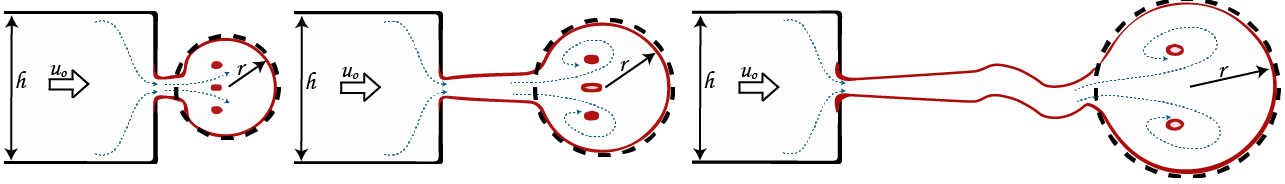
\includegraphics[width=1\linewidth]{Figures/VortexPair/model_100_200_400_3.png}
		\end{minipage}
		
		\caption{(a) Illustration of flow evolution through the narrow slit to an unbounded opening case. The dashed circle in each panel marks an approximation of the starting flow in a circular shape of radius $r$. A slug flow is assumed as inlet with velocity $u_o$ in a channel of width $h$.}
		\label{fig:model}
	\end{figure}

The present investigation sets out to explore the physics of fluid flow in a confined channel, with a specific emphasis on fluid dynamics at the exit past wall-mounted thin flexible plates. In both industrial and natural contexts, it is essential to comprehend the behavior of fluid flow in confined spaces, for instance, in pipeline systems and river beds. This understanding is further enhanced by studying the interactions between the fluid and solid structures within these confined channels. The current investigation employs a two-dimensional channel model to explore these dynamics, helping us to further our understanding of fluid-structure interaction problems.
\begin{figure}[h]
	\centering
	\begin{minipage}[c]{0.58\linewidth}
		\centering
		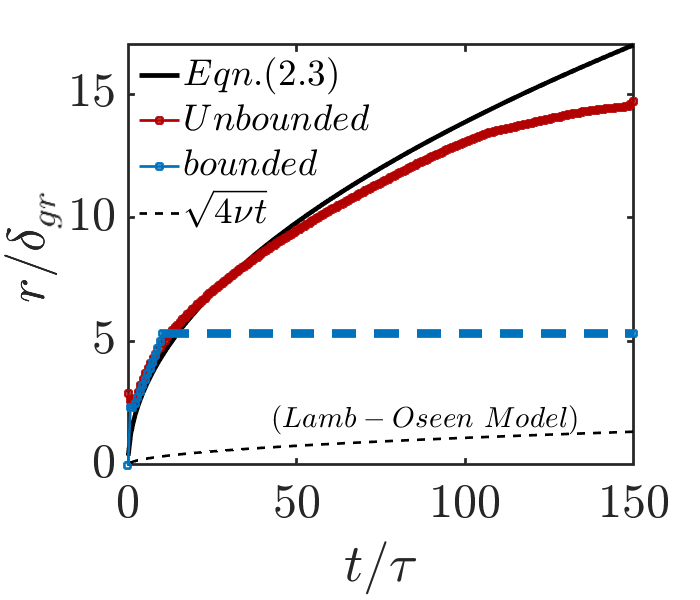
\includegraphics[width=1\linewidth] {Figures/radius_model2.png} 
	\end{minipage}
	\caption{Radius of the rolled-up starting flow evolution for the unbounded and bounded case with proposed growth model (solid black line) with time. A sample growth rate due to viscous diffusion (Lamb-Oseen Model) is shown in black dashed line for comparison.}
	\label{fig:model}
\end{figure}

Our study focuses on a channel of a certain height ($h$) and length ($14h$), in which two flexible plates are mounted on opposite walls at a certain distance ($2h$) from the channel inlet. The model's schematic can be seen in Figure \ref{fig:schematic}. Each plate has a length of $0.425h$ and is designed to be thin and flexible, with a thickness ($b$) of $0.05h$ and width ($w$) of $0.125h$ (into the plane). In real-world applications, these plates might represent structural elements like pipes, straws, or wall mounts in fluid-carrying systems, which often interact with the flow and lead to intriguing fluid dynamics and physical phenomena.

\begin{figure}[h]
	\centering
	\begin{minipage}[c]{0.77\linewidth}
		\vspace{0.7cm}
		\begin{overpic}[width=0.97\linewidth,height=1.5cm,trim=10 120 400 120, clip]{Figures/Figures/Jet/1S/1S_vort_100.png}
			\put(-25,20){{\parbox{0.4\linewidth}{$(a)$}}}
		\end{overpic}
		\begin{overpic}[width=0.97\linewidth,height=1.5cm,trim=10 120 400 120, clip]{Figures/Figures/Jet/1S/1S_vort_500.png}
			\put(-25,20){{\parbox{0.4\linewidth}{$(b)$}}}
			\put(160,24){{\parbox{0.4\linewidth}{$LVP$}}}
		\end{overpic}
%		\begin{overpic}[width=0.97\linewidth,height=1.5cm,trim=10 120 400 120, clip]{Figures/Figures/Jet/1S/1S_vort_1000.png}
%			\put(-25,20){{\parbox{0.4\linewidth}{$(c)$}}}
%		\end{overpic}
		\begin{overpic}[width=0.97\linewidth,height=1.5cm,trim=10 120 400 120, clip]{Figures/Figures/Jet/1S/1S_vort_1400.png}
			\put(-25,20){{\parbox{0.4\linewidth}{$(c)$}}}
			\put(80,29){{\parbox{0.4\linewidth}{$trailing \ shear \ layer$}}}
		\end{overpic}		
		\begin{overpic}[width=0.97\linewidth,height=1.5cm,trim=10 120 400 120, clip]{Figures/Figures/Jet/1S/1S_vort_1600.png}
			\put(-25,20){{\parbox{0.4\linewidth}{$(d)$}}}
		\end{overpic}
	\end{minipage}
	\begin{minipage}[c]{0.04\linewidth}
		\begin{overpic}[width=1\linewidth,height= 4.5cm]{Figures/Figures/Jet/leg_vort.png}
			\put(15,62){{\parbox{0.4\linewidth}{\rotatebox{90}{\Large$\Omega$}}}}
			\put(15,105){{\parbox{0.4\linewidth}{\Large$5$}}}
			\put(10,20){{\parbox{0.4\linewidth}{\Large$-5$}}}		
		\end{overpic}
		\vspace{0.2cm}
	\end{minipage}
	\caption{Contour of instantaneous vorticity contour of the flow through slit between the rigid plates. Time snapshots are at instances $t/\tau \approx 7,\ 36,\ 73,\ 103, \ and \ 117 $ for each panel respectively.}
	\label{fig:Vort_contour_1S}
\end{figure}

At the channel inlet, the flow profile is set to emulate a fully developed parabolic nature, represented by $u(y)=4u\left(\frac{y}{h}\right)\left(1-\frac{y}{h}\right)$. This formulation is based on the assumption of a steady laminar inlet flow in the channel, with a maximum inlet velocity $u_0$ at mid-channel height and a Reynolds number ($Re_\infty$) of $500$. The Reynolds number is calculated by the expression $Re_\infty={\rho_fu_o h}/\mu_f$, where $\rho_f$ is fluid density, and $\mu_f$ is fluid viscosity. The boundary conditions include a zero pressure gradient and a zero-velocity gradient at the channel outlet, ensuring minimal impact of the outlet boundary on the flow dynamics.

In addition to these primary conditions, certain specifications are designed to cater to the fluid-structure interactions in the channel. These include the application of no-slip conditions on the channel boundary walls and on the fluid-plate interface and setting the ratio of fluid density to structure density ($\rho_f / \rho_s$) at $0.02$. Moreover, the flexibility of the two plates, one of the key parameters of our study, is quantified using the Cauchy Number ($Ca$). The Cauchy number, expressed as $Ca=\rho_f u_o^2 h^3 b/{\mathcal{E}I} $, indicates the ratio between fluid inertial force and the structural restoring force of the plate. Here, $I=bw^3/12$ represents the area moment of inertia of the plate structure. The focus of our study is to compare wall-mounted rigid plates in channel with flexible plates ranging Cauchy number as low as $Ca=0.0008$ to $Ca = 0.06$. Our numerical setup includes discretization of the channel domain ($h\times14h$) into a grid of hexahedral cells (118 cells along the channel height and 520 cells along its length). We further discretize the thin plate structures into a hexahedral grid comprising 20 cells along the thickness and 80 cells along the plate height. To ensure the accurate and comprehensive interpretation of our results, we have considered a time scale factor based on convective motions at the narrow slit in rigid plate cases, $\tau={\delta_g/u_g}$, and simulated the results up to $t/\tau=600$.

The rest of the paper is structured as follows: section \ref{sec:Results} presents our results and discussion, with further sections providing detailed insight into various aspects of the study.

\section{Flow through slit past rigid plates}\label{sec:Results}

In this study we explore the fluid dynamics in a narrow, slit-like gap formed by two rigid, wall-mounted plates. This analysis is based on the interpretation of the velocity contour, delineated in Figure \ref{fig:Ux_contour_1S}, which provides an illustrative understanding of the flow process through this specific spatial configuration. The investigation focuses on a series of time frames, specifically $t/\tau \approx 7,\ 35,\ 70,\ and \ 103$, whose corresponding flow states are depicted in the sub-panels $(a)-(d)$ of the figure. The colour contours are scaled according to the streamwise velocity component normalised by initial inlet velocity at the channel centreline ($u_x/u_o$). At the initial stages, the fluid enters the slit gap-width $\delta_g$ and experiences acceleration due to the spatial confinement offered by the narrow slit. This acceleration instigates a roll-up motion perpendicular to the flow direction, leading to the formation of a "mushroom"-like structure at the head of the flow. This unique structure, comprising a counter-rotating vortex pair, is a key feature in such flows and is referred to as the 'leading vortex pair' (LVP). The LVP, once formed, sets out on a downstream journey, marking its path as the first mass ejection that emerges from the system. An interesting interaction unfolds as this LVP interacts with the slit. A trailing shear layer, evolving in congruity with the self-similar growth pattern of the LVP, connects the vortex pair with the slit edges and travels downstream. As seen in the subsequent panels of Figure \ref{fig:Ux_contour_1S}, the shear layer expands over time upto saturation limit. Past this limit, the attached trailing shear layer becomes unstable and begin to detach off from the LVP. Panel $(d)$ shows the 'detachment' instance of the leading fluid mass. However, the growth of this structure is regulated by the boundary conditions imposed by the channel walls.


\begin{figure}[h]
	\centering
	\begin{minipage}[c]{0.46\linewidth}
		\centering
		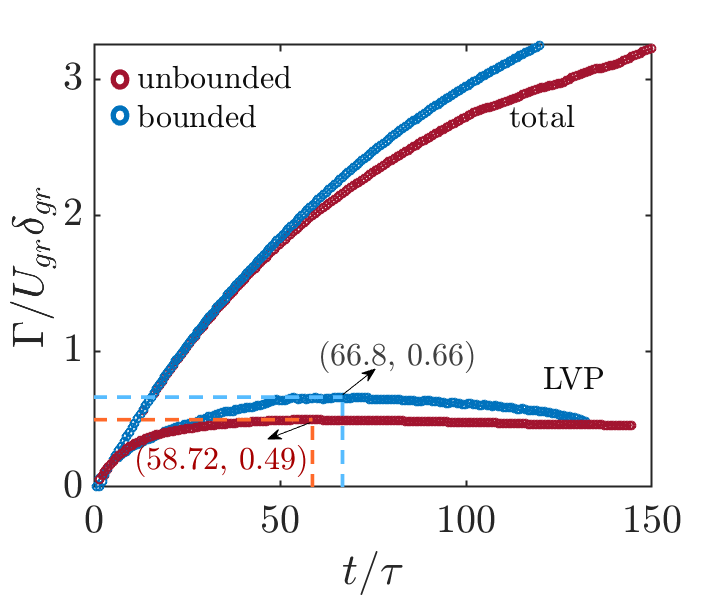
\includegraphics[width=1\linewidth] {Figures/Circ_S1.png} 
	\end{minipage}
	\begin{minipage}[c]{0.495\linewidth}
		\centering
		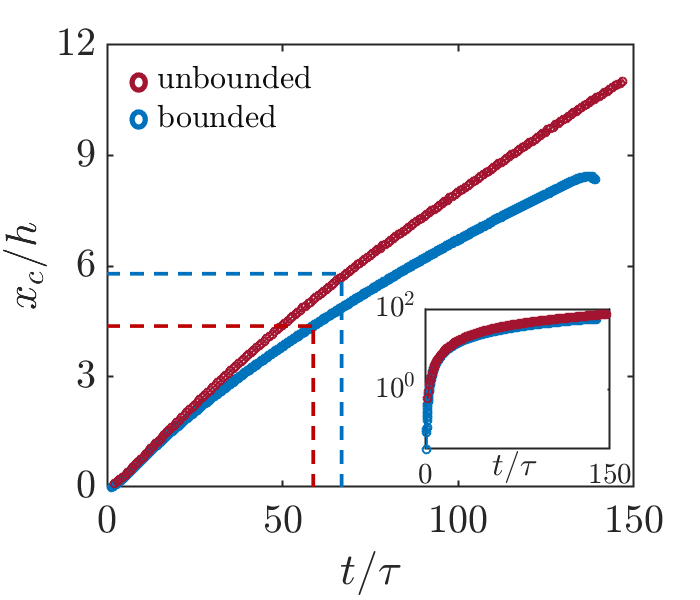
\includegraphics[width=1\linewidth] {Figures/velocity.png} 
	\end{minipage}
	\caption{(a) Time evolution of the vortex circulation, normalized by the velocity and width at the slit ($\Gamma$/$u_g\delta_g$) for net ejected flow and also for leading vortex pair (LVP). The dashed lines mark the maxima of the accumulated circulation within the LVP and hints its detachment.(b) Position trace of the leading vortex pair (LVP) for unbounded and bounded case. The subplot inside shows semi-log plot to show corresponding change in the position steepness.}
	\label{fig:Circ_S1_vs_T}
\end{figure}

\subsection{Comparative Analysis: Bounded and Unbounded Cases}\label{sec:comp_analysis}

To enhance our understanding of the system, we conduct a comparative analysis considering a fluid dynamic situation akin to our initial setup, but with wider channel openings. This scenario, portrayed in Figure \ref{fig:Ux_contour_1S_unbounded}, can be deemed to replicate an "unbounded" case. In this case, the growth of the fluid structure, specifically the mushroom-shaped ejection, is unimpeded by any channel walls, which contrasts with the in-channel or "bounded" flow situation. The figure shows normalised streamwise velocity contour at three different time instances. Panel $(b)$ of this figure provides a representative velocity vector field and vorticity outlines to facilitate the flow field visualisation. From the visual depiction, it is apparent that the ejection in the "unbounded" case grows significantly, unlike the confined growth observed in the "bounded" case. This observation highlights the impact of channel walls on flow dynamics, demonstrating how they restrict the growth and movement of the fluid structure.

Our analysis has mainly focuses on the early evolution of the flow and the formation of the LVP. The leading vortex pair, however, is not a stable entity and often succumbs to destabilization. As the flow advances further downstream, the LVP destabilizes, a process highlighted in panel $(c)$ of the same figure. To develop a more profound understanding of this phenomenon and the early flow development process, we propose a mathematical model presented in the following section.

\subsection{Mathematical Model: Formation and Growth of the Leading Vortex Pair}

 The leading mass ejection, resulting from the roll-up of a trailing shear layer connected to the slit, is assumed to draw in all the fluid entering the gap of the slit. This mushroom-shaped fluid mass upon formation is hypothesized to adopt an almost circular shape of radius $r$ and exhibit a degree of self-similar radial growth. However, as the trailing shear layer stretches over time, it develops an instability that halts its radial growth. The process is outlined in the schematic illustration provided in Figure \ref{fig:model}.

A crucial parameter in our model is the discharge coefficient, which is assumed to be 1. This assumption implies that the fluid volume ejected through the slit equates to the volume of fluid entering the channel. The model imagines the fluid entering the system as a column of fluid at velocity $u_o$ and ejecting through the slit of gap-width $\delta_g$ at an average sectional velocity at the slit $u_{gr}$. Over time, the total fluid discharged, denoted as $Q_{in}$, is defined mathematically by the following expression:

\begin{equation}
	Q_{in}=\int_{0}^{t}u_o hdt = \int_{0}^{t}u_{gr} \delta_{gr}dt
	\label{eqn:Q_in}
\end{equation}

This equation encapsulates the principle of conservation of mass by equating the volume of fluid entering the system (inlet) with the volume discharged over time.

Within the context of the leading vortex pair, the ejected fluid accumulates in the circular, disk-shaped blob due to the roll-up of the shear layers. This accumulation displays a self-similar growth pattern in terms of its radius, $r(t)$. This observation allows us to represent the volume flow rate stored in the leading vortex pair, $Q_{lvp}$, in the following manner:

\begin{equation}
	\int_{0}^{t}Q_{lvp}dt= \pi r^2(t)
	\label{eqn:Q_lvp}
\end{equation}

In the above equation, the integral of the volume flow rate over time gives the volume of the fluid collected in the LVP. This is geometrically equivalent to the volume of a disk of radius $r(t)$.

By making two crucial assumptions: no entrainment effects (i.e., no additional fluid is drawn into the flow beyond what enters the slit) and a negligible trailing layer volume, we can infer that the volume flow rate entering the slit equals the volume flow rate stored in the LVP, i.e., $Q_{in}$ $=$ $Q_{lvp}$. This allows us to derive the growth of the leading vortex pair, linking it with the equations \ref{eqn:Q_in} and \ref{eqn:Q_lvp}, which results in the following relationship:

\begin{equation}
	r(t) = \sqrt{\frac{u_o h}{\pi}t}
	\label{eqn:r_lvp}
\end{equation}

This expression encapsulates the essence of our model, capturing the radius of the leading vortex pair as a function of time, $r(t)$, in terms of the inlet velocity $u_o$, channel height $h$, and time $t$. This model offers an analytical framework to understand the behavior of the leading vortex pair during the early stages of flow through a narrow slit. 



\begin{figure}
	\centering
	\begin{minipage}[c]{0.495\linewidth}
		\centering
		\begin{overpic}[width=1\linewidth]{Figures/Figures/time-space_S1_fixbc.png}
			\put(135,40){{\parbox{0.4\linewidth}{\rotatebox{0}{$unbounded$}}}}
			\put(70,65){{\parbox{0.1\linewidth}{\rotatebox{30}{$LVP$}}}}	
		\end{overpic}
	\end{minipage}
	\begin{minipage}[c]{0.495\linewidth}
		\centering
		\begin{overpic}[width=1\linewidth]{Figures/Figures/time-space_S1.png}
			\put(145,40){{\parbox{0.3\linewidth}{\rotatebox{0}{$bounded$}}}}
			\put(68,68){{\parbox{0.1\linewidth}{\rotatebox{40}{$LVP$}}}}
			%		\put(15,105){{\parbox{0.4\linewidth}{\Large$2.5$}}}
			%		\put(10,20){{\parbox{0.4\linewidth}{\Large$-2.5$}}}		
		\end{overpic}
	\end{minipage}
	\caption{Space-time map of the vertically integrated vorticity for bounded case. The continuous line is the automatically detected centre of the separated vortex, the dashed lines are the estimated vortex boundaries.}
	\label{fig:time_space}
\end{figure}

To illustrate the derived relation between the radius growth with respect to time, figure \ref{fig:model} shows the curve as a black line for the equation \ref{eqn:r_lvp}. We present the growth of the leading head for both bounded and unbounded starting flow through the slit. In the case of the unbounded flow evolution, the radius growth trend aligns with the proposed relation up to an initial time period, but at later times, the growth trend deviates. This deviation results from the no-entrainment and negligible trailing flow assumptions for the model proposition, which begin to fail as the flow extends longer into the downstream. For the bounded in-channel flow evolution, the initial growth seems to follow the proposed relation. However, due to the wall confinements in either direction, this growth gets hindered, and the leading patch no longer remains a circular disk. Instead, it extends laterally under the effect of wall boundaries. The growth curve for the bounded case is shown in the same figure as a blue line. The thick dashed blue line marks the channel width in the plot, which indicates the growth limits. We have also shown a typical viscous diffusion rate of a Lamb-Oseen vortex with constant circulation as a standard reference for comparison. This diffusion-based growth rate is much lower than in the present case of attached shear layer-based influx growth. 

	\begin{figure}[h]
	\begin{center}
		\begin{minipage}[c]{0.49\linewidth}	
			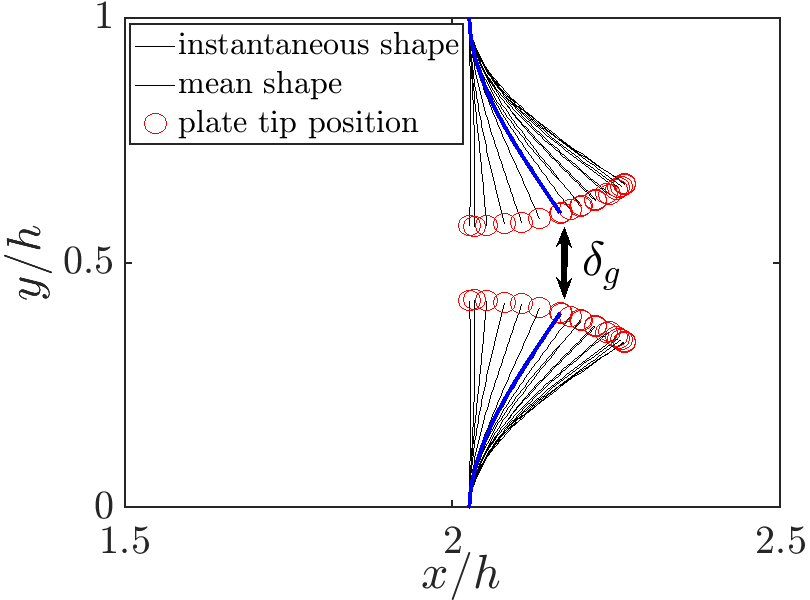
\includegraphics[width=1\linewidth]{Figures/def_shape2.png}\\
			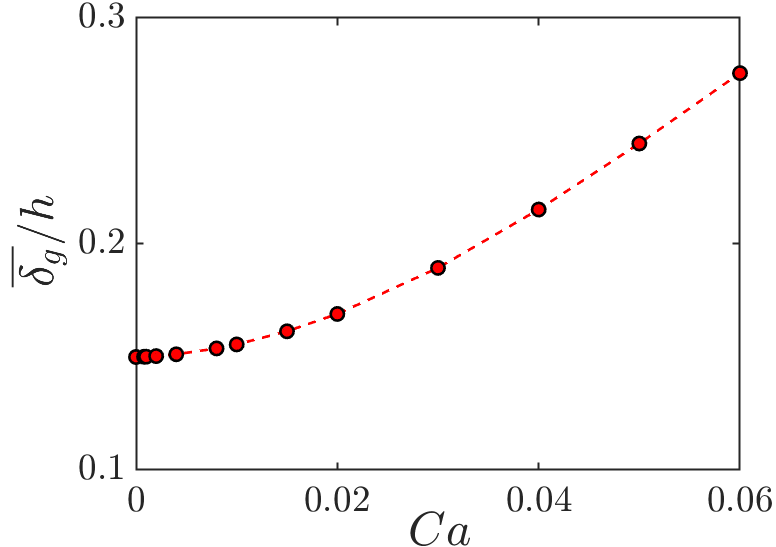
\includegraphics[width=1\linewidth]{Figures/gap_signal/gap_steady2.png}
		\end{minipage}
		\begin{minipage}[c]{0.49\linewidth}	
			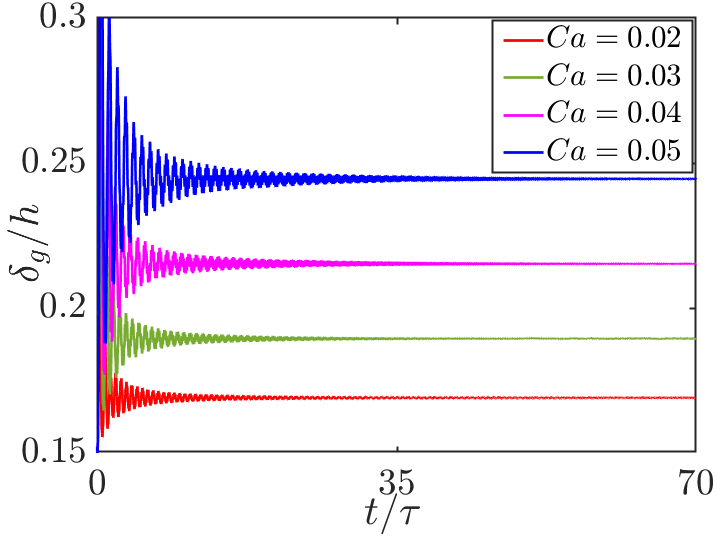
\includegraphics[width=1\linewidth]{Figures/gap_signal/gap_sig_3_4p1_5_5p1S-2.png}
			\begin{overpic}[width=0.95\linewidth]{Figures/drag/Cd_parabolic_S.png}
				\put(-230,335){{\parbox{1\linewidth}{$(a)$}}}	
				\put(-0,335){{\parbox{1\linewidth}{$(b)$}}}
				\put(-230,165){{\parbox{1\linewidth}{$(c)$}}}	
				\put(0,165){{\parbox{1\linewidth}{$(d)$}}}
			\end{overpic}
		\end{minipage}
	\end{center}
	\vspace{-10px}
	\caption{(a) Stroboscopic representation of the flexible plate deflection for a sample case. The slit gap ($\delta_g$) between the two plates increases as the plate deflects more under the flow. The thick blue line marks the mean position of the plate. (b) Time history of slit gap width normalized by the channel height ($\delta_g/h$) for plates with varying flexibility (i) $Ca=0.008$ (ii) $Ca=0.02$ (iii) $Ca=0.04$. (c) Trend of the mean slit gap width over the oscillatory steady state for different $Ca$.
		(a) Coefficient of drag ($Cd$) offered by the plates normalized by the drag offered by rigid plates.}
	\label{fig:del_g_vs_Ca_steady}
\end{figure}


 \subsection{Vortex pair roll-up}
To illustrate the vortex pair roll-up, we present the vorticity ($\Omega$) contour for the flow through the slit from rigid plates in Figure \ref{fig:Vort_contour_1S} at different time instants. Time snapshots are at instances $t/\tau \approx 7,\ 36,\ 73,\ 103, \ and \ 117 $ for each panel, respectively. The vorticity contour indicates the rotational direction of the flow: red denotes a counter-clockwise rotation, and blue indicates a clockwise rotation (the contour is identified at  $\approx  5\%$ of maximum vorticity). The figure captures the vorticity roll-up near the slit gap and its streamwise extension into the downstream over time. The leading vorticity pair as it grows is fed over time through the trailing shear layer. The separated flow off the plates' tip, at the narrow slit, induce velocity gradients into the flow which in turn generate vorticity. After a certain length of extension, the shear layer triggers Kelvin-Helmholtz instability, and the LVP begins to dissociate from its tail (see Figure \ref{fig:Vort_contour_1S} (d)). The detached pair no longer receives vorticity anymore from the tip attached shear layer. The LVP beyond this time and space begins to decay as it propagates into the downstream. Additionally, the effect of wall confinement can be observed as some vorticity is generated on either wall near the LVP. The wall confinement increases the fluid shear, which generates larger vorticity. 

In Figure \ref{fig:Circ_S1_vs_T}(a), we present the total circulation released off the rigid plates' edges for both bounded and unbounded cases. We calculate this circulation by considering the positive half of the vorticity in the complete downstream domain past the slit gap. We normalize the circulation by the slit gap-width and the mean velocity through the slit-gap to derive a non-dimensional scaling factor ($\Gamma/u_{gr}\delta_{gr}$). The figure shows that the bounded case accumulates more circulation over time compared to the unbounded case. This increased circulation is a consequence of the confined walls, which induce additional velocity gradients into the domain from either sides compared to those in the unbounded case. The same figure also shows the circulation entrapped in the flow head or the leading vortex (LVP). The results reflect a similar trend as seen in the case of total circulation, as the leading vortex pair grows and approaches the walls, thereby generating more shear against the wall boundaries. However, this process of accumulating vorticity from the inlet source does not continue indefinitely; the LVP attains a maximum circulation value. We mark this point with a dashed line in the same figure, which indicates the start-up time of the LVP. The start-up time for the bounded and unbounded cases is approximately $68$ and $\approx \ 59$, respectively. From these observations, we can conclude that the bounded in-channel setting delays the start-up time of the vortex pairs and draws more vorticity into them. The LVP at this point detaches from the attached trailing layer due to the aforementioned K-H instability. The dissociated LVP begins to decay past this start-up time, and the vortex core deviates from its rectilinear trajectory at a later time instant. The counter-rotating vortex pairs are self-propagating, and hence they continue to travel even after their dissociation, albeit at a slower rate. 
Figure \ref{fig:Circ_S1_vs_T}(b) shows the position track of the leading vortex core normalized over  $(xc)$ over time. The figure reveals that the traverse rate of the vortex core is slower than that in the unbounded domain case. As explained earlier, the boundary walls induce additional shear onto the LVP and thus resist the rate of its downstream propagation. Furthermore, the vortex pair also shows a gradual change in the rate of propagation based on their startup phenomena. The dashed line in the same figure marks the start-up time. As discussed previously, the induction of vorticity in the vortex pair stops at the start-up time, and thus no longer receives any direct inertial force from the inlet. Still, under the effect of advection and due to the self-propagating nature of the dipole, the LVP moves at a slightly lower rate. The sub-panel in the figure shows a semi-log plot for the same with the vortex core downstream position on a logarithmic scale. We have only shown the LVP until it is distinctly identifiable, but as the shear layer instability takes effect at later times, the rotating and counter-rotating part of the LVP arranges in alternating fashion in the downstream which also follows for subsequent  vortex pairs and their detachment.

Figure \ref{fig:time_space} shows the space-time map of the vertically integrated vorticity for unbounded and bounded cases in the left and right panel, respectively. The vorticity pattern in this figure imprints the trail of LVP  over time. After the LVP dissociates from the trailing shear layer, subsequent vortices form behind it. The imprint of these can be seen in the space-time map as fringe patterns, which correspond to the arrangement of dissociated vortices in alternating fashion. An early lateral spread of these released vortices is a noticeable difference in the case of the unbounded case compared to the bounded case.


\begin{figure}
	\centering
	\begin{minipage}[c]{0.77\linewidth}
		\vspace{0.7cm}
		\begin{overpic}[width=0.97\linewidth,height=1.5cm,trim=10 120 600 120, clip]{Figures/Figures/Jet/1S/4p1S_0050.png}
			\put(-25,20){{\parbox{0.4\linewidth}{$(a)$}}}
		\end{overpic}
		\begin{overpic}[width=0.97\linewidth,height=1.5cm,trim=10 120 600 120, clip]{Figures/Figures/Jet/1S/4p1S_0100.png}
			\put(-25,20){{\parbox{0.4\linewidth}{$(b)$}}}
			%				\put(160,24){{\parbox{0.4\linewidth}{$LVP$}}}
		\end{overpic}
		\begin{overpic}[width=0.97\linewidth,height=1.5cm,trim=10 120 600 120, clip]{Figures/Figures/Jet/1S/4p1S_0150.png}
			\put(-25,20){{\parbox{0.4\linewidth}{$(c)$}}}
		\end{overpic}
		\begin{overpic}[width=0.97\linewidth,height=1.5cm,trim=10 120 600 120, clip]{Figures/Figures/Jet/1S/4p1S_0300.png}
			\put(-25,20){{\parbox{0.4\linewidth}{$(d)$}}}
			\put(360,5){{\parbox{0.4\linewidth}{$Ca=0.03$}}}
		\end{overpic}		
	\end{minipage}
	\begin{minipage}[c]{0.04\linewidth}
		\begin{overpic}[width=1\linewidth,height= 4.5cm]{Figures/Figures/Jet/leg_vort.png}
			\put(15,62){{\parbox{0.4\linewidth}{\rotatebox{90}{\Large$\Omega$}}}}
			\put(15,105){{\parbox{0.4\linewidth}{\Large$5$}}}
			\put(10,20){{\parbox{0.4\linewidth}{\Large$-5$}}}		
		\end{overpic}
		\vspace{0.2cm}
	\end{minipage}
	\caption{Contour of instantaneous vorticity contour of the flow through slit between the flexible plates with $Ca=0.03$. Time snapshots are at instances $t/\tau \approx 3,\ 7,\ 11,\ and \ 22 $ for each panel respectively.}
	\label{fig:Vort_contour_4S}
\end{figure}



\begin{figure}[h]
	\centering
	\begin{minipage}[c]{0.65\linewidth}
		\begin{overpic}[width=1\linewidth, trim=10 119 900 119,clip]{Figures/Figures/Jet/vort/1S_0300.png}
			\put(-50,20){{\parbox{1\linewidth}{$rigid$}}}
		\end{overpic}
		\begin{overpic}[width=1\linewidth, trim=10 119 900 119,clip]{Figures/Figures/Jet/vort/2p3S_0300.png}
			\put(-58,20){{\parbox{1\linewidth}{$Ca=0.001$}}}
		\end{overpic}
		\begin{overpic}[width=1\linewidth, trim=10 119 900 119,clip]{Figures/Figures/Jet/vort/3p1S_0300.png}
			\put(-58,20){{\parbox{1\linewidth}{$Ca=0.015$}}}
		\end{overpic}
		\begin{overpic}[width=1\linewidth, trim=10 119 900 119,clip]{Figures/Figures/Jet/vort/4S_0300.png}
			\put(-58,20){{\parbox{1\linewidth}{$Ca=0.02$}}}
		\end{overpic}
		\begin{overpic}[width=1\linewidth, trim=10 119 900 119,clip]{Figures/Figures/Jet/vort/4p1S_0300.png}
			\put(-58,20){{\parbox{1\linewidth}{$Ca=0.03$}}}	
		\end{overpic}
		\begin{overpic}[width=1\linewidth, trim=10 119 900 119,clip]{Figures/Figures/Jet/vort/5S_0300.png}	
			\put(-58,20){{\parbox{1\linewidth}{$Ca=0.04$}}}		
		\end{overpic}
		\begin{overpic}[width=1\linewidth, trim=10 119 900 119,clip]{Figures/Figures/Jet/vort/6S_0300.png}	
			\put(-58,20){{\parbox{1\linewidth}{$Ca=0.06$}}}		
		\end{overpic}
	\end{minipage}
	\caption{Instantaneous vortex contour for steady inflow past the slit for cases with rigid plates and flexible plate cases with $Ca=0.0008$ to $Ca=0.06$. (top to bottom). See Animation 1 in supplementary attachment.}
	\label{fig:Vort_Ca}
\end{figure}


\section{Flow through slit past flexible plates}\label{sec:flex_plate_dynamics}

Having understood the evolution and dynamics of the LVP with rigid plates forming the slit, it is worth investigating how flexible plates can affect vortex generation. As we aim to induce early dissociation or pinch-off phenomena in vortex pair cases, flexible plates are an interesting variant to consider. These plates, when confronted with an incoming flow, gradually deform, driven by the prevailing fluid inertia overpowering their bending stiffness \citep{Shelley2011}. Consequently, their structure reshapes into a streamlined form, reducing the projected area perpendicular to the flow and thus mitigating the overall drag force. Our investigation reveals this structural transformation of flexible plates under the effect of a parabolic inlet flow profile, as depicted in Figure \ref{fig:del_g_vs_Ca_steady}(a). Utilizing stroboscopic visualization, the preliminary transients of the plates' reshaping are evident. This figure corresponds to a scenario with $Ca = 0.04$ and a steady incoming flow at $Re=500$. The plates undergo bending along their length, exhibiting maximum deflection at their free end or tip, depicted by the red circles over the thin black time sequence of plate positions. Initially, within the transient state, the plates experience considerable deformation along the incoming flow direction, reaching approximately half their length. However, a steady-state inlet situates the plates in a mean position, prompting oscillations around this average position. The thick blue shape of the plates in the figure represents this mean position.

The two plates, mounted in opposition, resemble a two-dimensional narrow slit for flow entry. However, for the flexible plate model, the system can be approximated as a slit with a varying opening size (gap) over time. This variation hinges on the inlet flow frequency and other intricate dynamics, which we will dissect in subsequent sections. The mean gap width, denoted as $\delta_g$, representing the distance between the tips of the two plates in their mean position (thick blue line in Figure \ref{fig:del_g_vs_Ca_steady}(a)), fluctuates in response to the fluid forces at the inlet versus the structural forces acting upon the plates as cantilever loads, as previously discussed. In-depth analysis of the structural behavior of these plates under uniform flow conditions was previously undertaken in our prior work \citep{Self2019}. In this work, we likened the wall-mounted plates to a typical spring-mass-damper model, approximating the vibration analysis, including the damping of plate oscillations from transient to steady-state. Figure \ref{fig:del_g_vs_Ca_steady}(b) presents the temporal signal variation of the slit opening ($\delta_g$), normalized by the channel height ($h$), for different cases of plate flexibility ($Ca$) under steady flow conditions. Intriguingly, all three cases manifest flutter instability at the tip of the plates even within a steady flow inlet environment. However, these time signals ultimately reach an oscillatory steady-state condition over time. The mean of this oscillatory steady state for the slit opening ($\overline{\delta_g}$) is found to scale with increasing plate flexibility, i.e., $Ca=0.0008$ to $Ca=0.06$, as depicted in Figure \ref{fig:del_g_vs_Ca_steady}(c). The figure demonstrates a nonlinear increase in slit width and plates' flexibility ($Ca$).

In Figure \ref{fig:del_g_vs_Ca_steady}(d), the drag coefficient normalised by the same in rigid plate case ($C_d=F_d/0.5\rho_f u_o^2$, where $F_d$ signifies the drag force encountered) is depicted at the steady-state reconfigured duration of the simulation. On comparing the mean drag experienced by the flexible plates versus the rigid plate scenario, an increment in mean drag is observed until the maximum drag occurring at approximately $Ca=0.01$, as shown in Figure \ref{fig:del_g_vs_Ca_steady}(c). This is attributed to the formation of a stagnant fluid region behind the plates that enhance their resistance against the incoming fluid inertia. Beyond this regime, i.e., for $Ca>0.01$, the fluid behind the plates becomes somewhat perturbed, intensifying the plates' motion to become more compliant and less resistant. Consequently, the mean drag diminishes as plates' flexibility increases. This phenomenon underscores the intricate interplay between flexible plates and fluid dynamics, ultimately impacting vortex pair formation and pinch-off behaviors.



\begin{figure}[h]
	\centering
	\begin{minipage}{0.65\linewidth}
		\begin{overpic}[width=1\linewidth]{Figures/velpro/1S_parabolic_velpro.png}
			\put(-20,0){{\parbox{0.4\linewidth}{$(a)$}}}
		\end{overpic}
		\begin{overpic}[width=1\linewidth]{Figures/velpro/1S_parabolic_umean.png}
		\end{overpic}
		\begin{overpic}[width=1\linewidth]{Figures/velpro/4S_parabolic_velpro.png}
			\put(-20,0){{\parbox{0.4\linewidth}{$(b)$}}}
		\end{overpic}
		\begin{overpic}[width=1\linewidth]{Figures/velpro/4S_parabolic_umean.png}
		\end{overpic}
		\begin{overpic}[width=1\linewidth]{Figures/velpro/6S_parabolic_velpro.png}
			\put(-20,0){{\parbox{0.4\linewidth}{$(c)$}}}
			%	\put(30,-0){{\parbox{0.4\linewidth}{$x/h$}}}
		\end{overpic}
		\begin{overpic}[width=1\linewidth]{Figures/velpro/6S_parabolic_umean.png}
		\end{overpic}
		\begin{overpic}[width=1\linewidth]{Figures/midline/S_midline_parabolic.png}
			\put(155,-10){{\parbox{1\linewidth}{$x/h$}}}
			\put(-20,22){{\parbox{0.4\linewidth}{$(d)$}}}
		\end{overpic}
	\end{minipage}
	\begin{minipage}{0.07\linewidth}
		\begin{overpic}[width=0.7 \linewidth]{Figures/velpro/legend.png}
		\end{overpic}
	\end{minipage}
	\vspace{0.1cm}
	\caption{Time-averaged velocity profiles across the channel at
		nine streamwise locations and time-averaged flow field for plates with varying flexibility cases for (a)rigid (b)$Ca=0.02$, and (c) $Ca=0.06$. (d) Time-averaged centerline Reynolds number ($Re_c$) along the channel’s length normalized by inlet Reynolds number ($Re_\infty$). To guide the eye, dashed horizontal line show the inlet flow $Re_\infty$.}
	\label{fig:velpro_mean}
\end{figure}



\begin{figure}[h]
	\centering
	\begin{minipage}[c]{0.49 \linewidth}
		\centering
		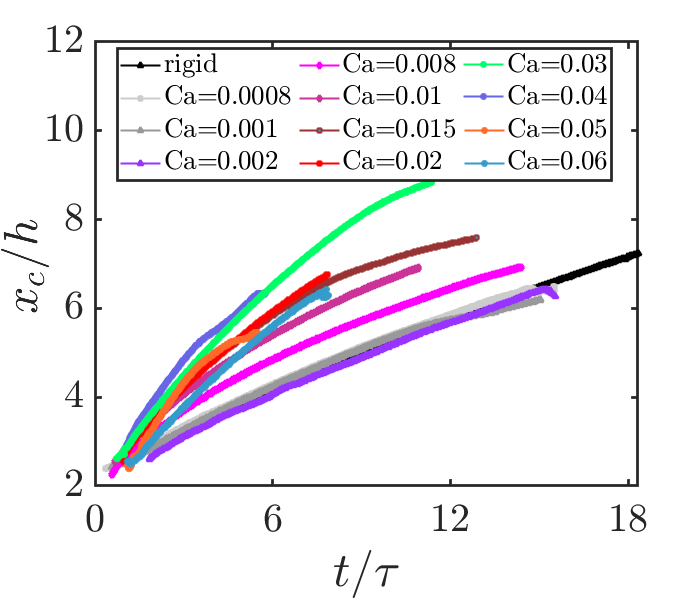
\includegraphics[width=1\linewidth] {Figures/vortProp/vortprop_S_parabolic.png} 
	\end{minipage}
	\begin{minipage}[c]{0.49\linewidth}
		\centering
		%	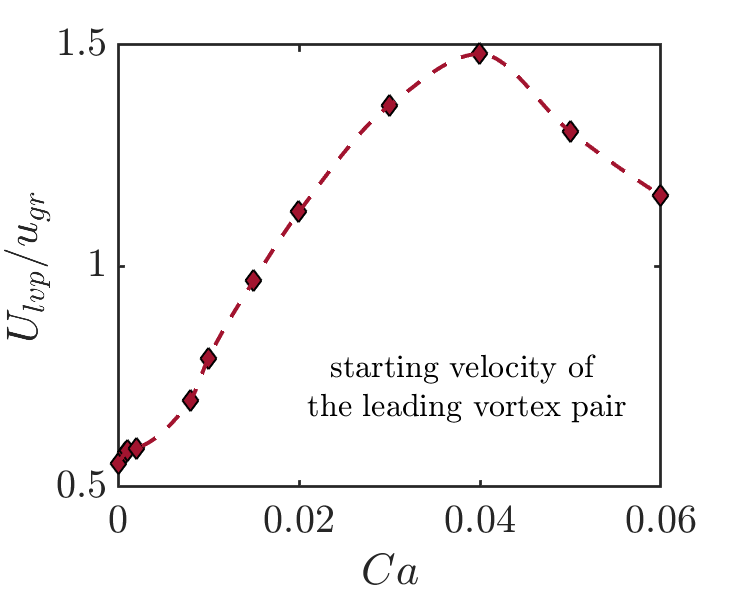
\includegraphics[width=0.985\linewidth] {Figures/vortProp/S_slope.png} 
		\begin{overpic}[width=1\linewidth] {Figures/vortProp/S_slope.png} 
			\put(-240,195){{\parbox{1\linewidth}{$(a)$}}}	
			\put(-5,195){{\parbox{1\linewidth}{$(b)$}}}	
		\end{overpic}
	\end{minipage}
	\caption{Position track of the ejected leading vortex pair over time for the range of $Ca$. (b) Corresponding slope (or starting velocity) for different $Ca$ cases. Maxima of the velocity of the vortex pair at $Ca=0.03$ can be observed.}
	\label{fig:vortPnC}
\end{figure}
\subsection{Impact of plate flexibility on flow features}
As our study progresses, subsequent sections will delve deeper into the complex dynamics governing these phenomena, unravelling the interdependencies between plate flexibility, fluid forces, and the resulting flow patterns. When flexible plates are used instead of rigid plates to form a narrow slit, the flow evolution is significantly different. For an illustration, Figure \ref{fig:Vort_contour_4S}$(a)-(d)$ shows instantaneous vorticity contours for a flexible plate case ($Ca=0.03$) at subsequent time instances, i.e., $t/\tau=3,\ 7,\ 11,\ and \ 22$, respectively. As the flexible plate reconfigures according to the inlet fluid load, the starting flow shows a similar mushroom-shaped leading blob of flow immediately after the slit gap width. However, this LVP dissociates from the plate attached shear layer much earlier than in the rigid plate case. Furthermore, this LVP travels longer into the downstream after its dissociation. This phenomenon appears to be similar to "pinch-off", which was previously found to be absent in the case of a 2D vortex pair system \cite{pedrizzetti_2010, Afanasyev2006}. After the pinch-off of the LVP, a secondary vortex pair ejects off the plates' edges in succession, as can be seen in Figure \ref{fig:Vort_contour_4S}(b). The secondary vortex pair also pinches off in a similar fashion, and another vortex pair lines up at the slit opening. At a certain time, a train of vortex pairs can be observed along the channel length, as shown in panel $(d)$ of the same figure. Interestingly, the use of flexible plates for a narrow slit induces a pinch-off phenomenon in two-dimensional starting flows and, moreover, a periodic generation of vortex pairs.


\begin{figure}[h]
	\centering
	\begin{minipage}[c]{0.24\linewidth}
		\centering
		%	(a)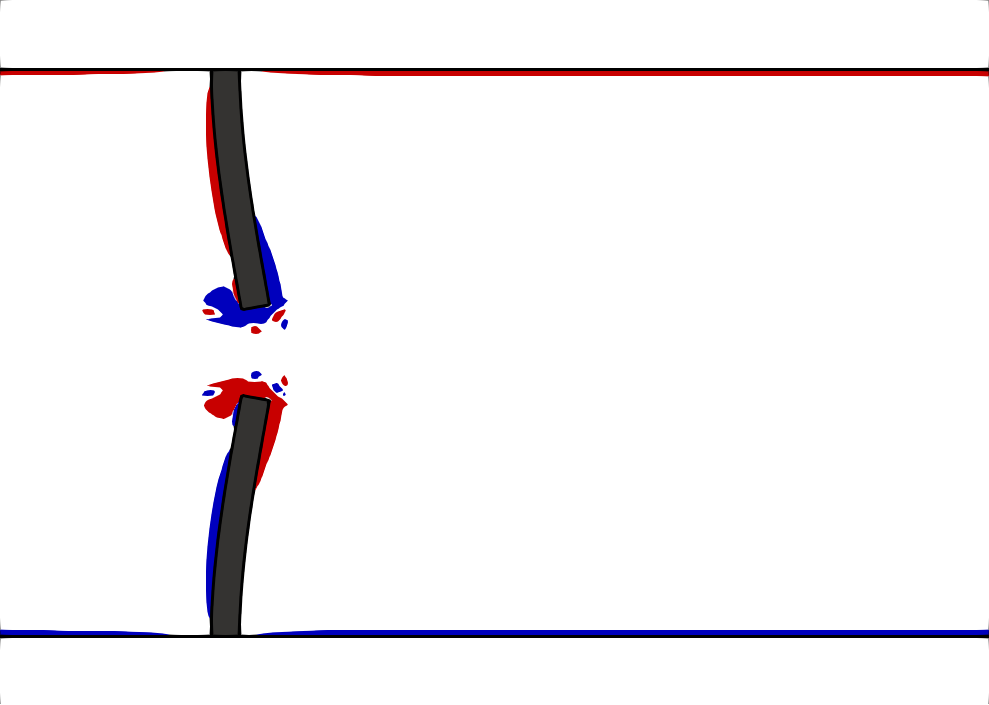
\includegraphics[width=0.7\linewidth]{Figures/5C_selected/5C0006.png}
		\begin{overpic}[width=1\linewidth]{Figures/VortexEvol/1S/1S0015.png}
			\put(0,80){{\parbox{0.4\linewidth}{$(a)$}}}
			\put(-15,37){{\parbox{0.4\linewidth}{$rigid$}}}
		\end{overpic}
		\begin{overpic}[width=1\linewidth]{Figures/VortexEvol/4S/4S0015.png}
			\put(0,60){{\parbox{0.4\linewidth}{$(e)$}}}
			\put(-20,37){{\parbox{1\linewidth}{$Ca=0.02$}}}
		\end{overpic}
		\\$t/\tau=1$
	\end{minipage}
	\begin{minipage}[c]{0.24\linewidth}
		\centering
		%	(a)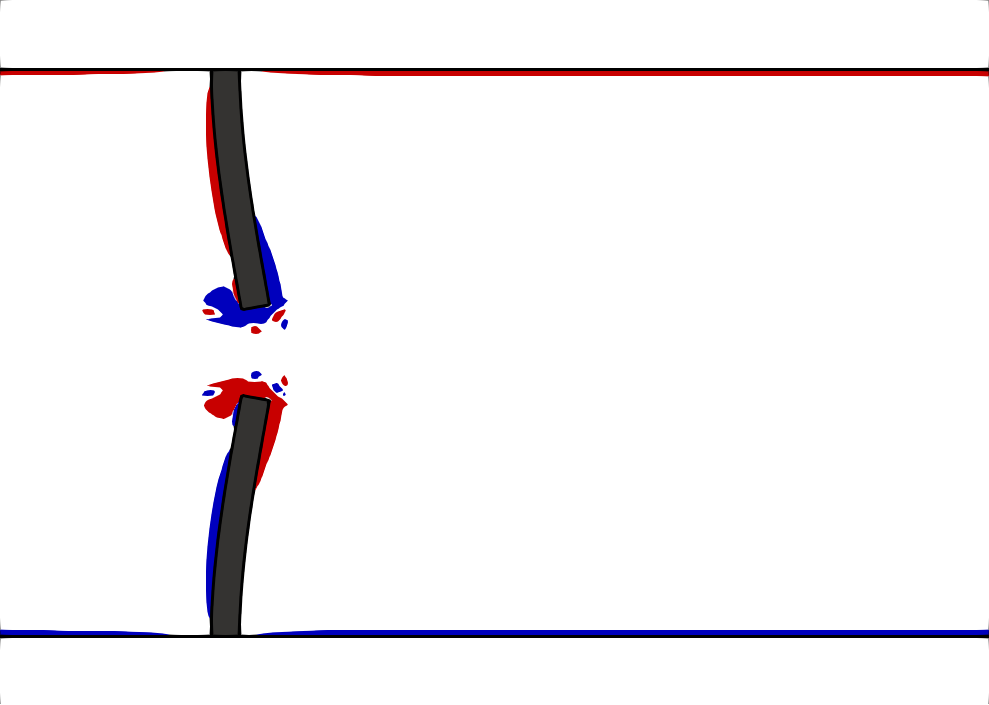
\includegraphics[width=0.7\linewidth]{Figures/5C_selected/5C0006.png}
		\begin{overpic}[width=1\linewidth]{Figures/VortexEvol/1S/1S0025.png}
			\put(0,80){{\parbox{0.4\linewidth}{$(b)$}}}
			%		\put(-75,30){{\parbox{0.4\linewidth}{$t/\tau=0.15$}}}
		\end{overpic}
		\begin{overpic}[width=1\linewidth]{Figures/VortexEvol/4S/4S0025.png}
			\put(0,60){{\parbox{0.4\linewidth}{$(f)$}}}
			%			\put(-75,30){{\parbox{0.4\linewidth}{$t/\tau=0.25$}}}
		\end{overpic}
		\\$t/\tau=1.85$
	\end{minipage}
	\begin{minipage}[c]{0.24\linewidth}
		\centering
		%	(a)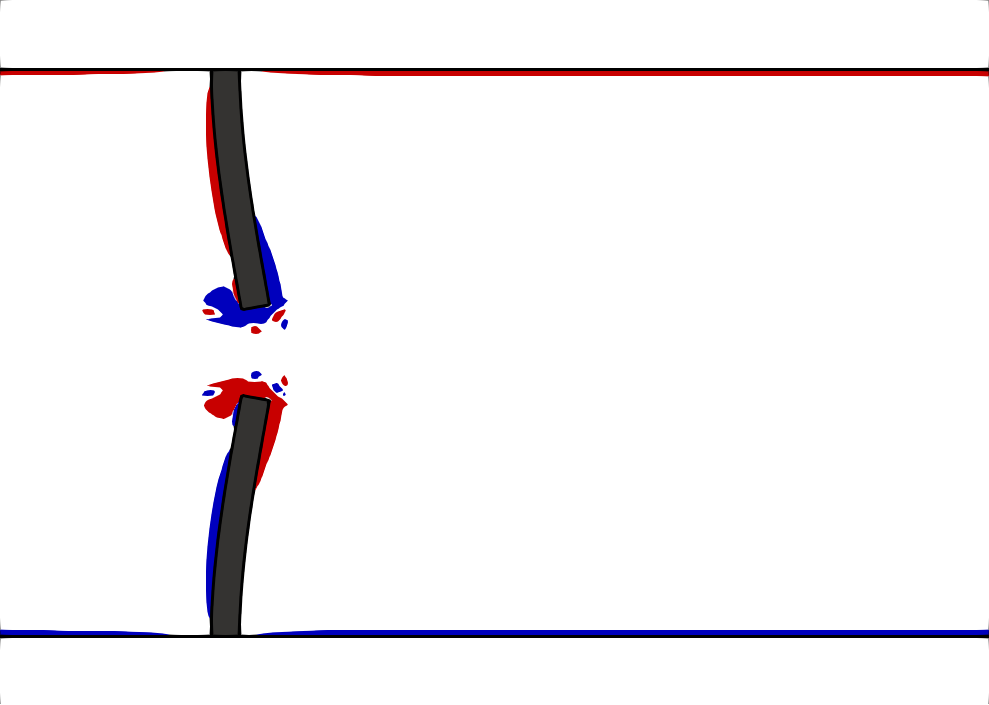
\includegraphics[width=0.7\linewidth]{Figures/5C_selected/5C0006.png}
		\begin{overpic}[width=1\linewidth]{Figures/VortexEvol/1S/1S0045.png}
			\put(0,80){{\parbox{0.4\linewidth}{$(c)$}}}
			%		\put(-75,30){{\parbox{0.4\linewidth}{$t/\tau=0.15$}}}
		\end{overpic}
		\begin{overpic}[width=1\linewidth]{Figures/VortexEvol/4S/4S0045.png}
			\put(0,60){{\parbox{0.4\linewidth}{$(g)$}}}
			%		\put(-75,30){{\parbox{0.4\linewidth}{$t/\tau=0.25$}}}
		\end{overpic}
		\\$t/\tau=3.30$
	\end{minipage}
	\begin{minipage}[c]{0.24\linewidth}
		\centering
		%	(a)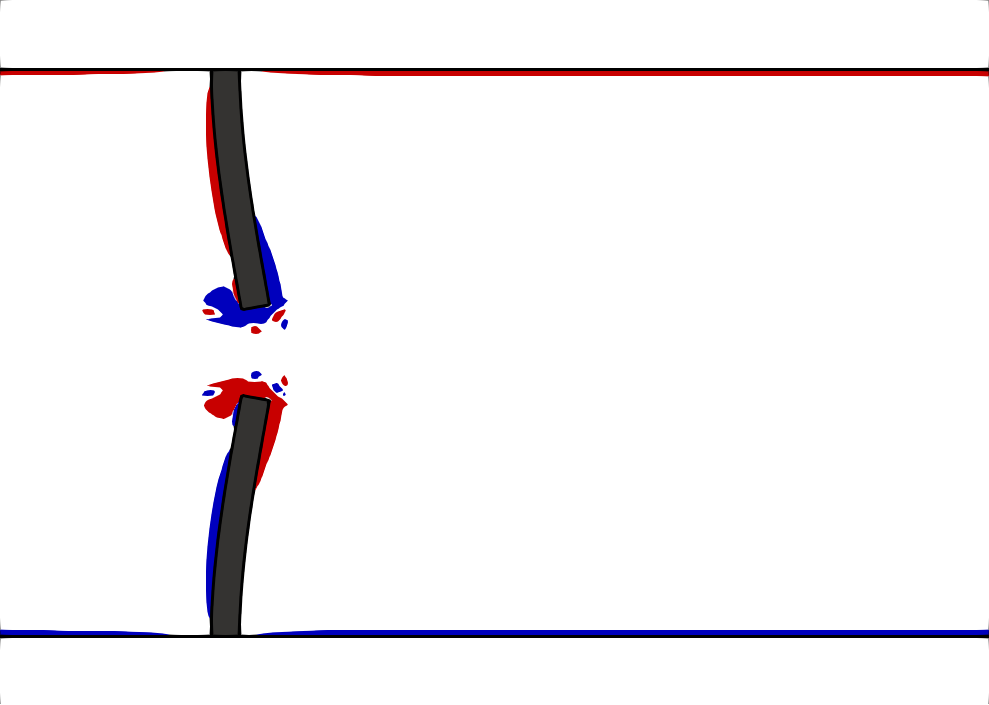
\includegraphics[width=0.7\linewidth]{Figures/5C_selected/5C0006.png}
		\begin{overpic}[width=1\linewidth]{Figures/VortexEvol/1S/1S0065.png}
			\put(0,80){{\parbox{0.4\linewidth}{$(d)$}}}
			%		\put(-75,30){{\parbox{0.4\linewidth}{$t/\tau=0.15$}}}
		\end{overpic}
		\begin{overpic}[width=1\linewidth]{Figures/VortexEvol/4S/4S0065.png}
			\put(0,60){{\parbox{0.4\linewidth}{$(h)$}}}
			%		\put(-75,30){{\parbox{0.4\linewidth}{$t/\tau=0.25$}}}
		\end{overpic}
		\\$t/\tau=4.75$
	\end{minipage}
	\caption{Comparison of starting vortex ejection rigid and flexible plate case. (a) Time sequence of vorticity contours for (a-d) rigid plate case and (e-h) flexible plate case, $Ca=0.02$. The blue and red colour shows clockwise and counter-clockwise vortices respectively}
	\label{fig:vort_evo_1S_4S}
\end{figure}

To further investigate the effect of plate flexibility, we compare cases with different $Ca$ in Figure \ref{fig:Vort_Ca}. Vorticity contours at a time instant $t/\tau=22$ are shown for the rigid plate case (topmost panel) to the most flexible plate case in our simulations (bottom-most panel). A qualitative overview instantly compares the effect of flexible plates with that of rigid plate case. The rigid plate case shows a stable self similar growth of the trailing shear layer and the LVP. On the contrary, a slight increase in plates' flexibility $Ca=0.001$ cause incoherent growth in vorticity structure. Also, a pair of rolled-up vortices can be seen behind the plates' fixed ends in the form of corner trapped structures. The unstable shear layer causes an early dissociation of the LVP. Another slight increase in plates' flexibility $(Ca=0.015)$ generates propulsive LVP with much early pinch-off. The pinched-off LVP takes a lead and travels much ahead than the attached trailing shear layer flow. In the similar trend, the LVP in higher $Ca$ cases appear to gain larger propulsion off the plates' oscillation. The LVP dissociates of the plate attached shear layer with additional roll-ups as second and third vortex pairs generated in sequence. Another interesting feature to note is the backflow into the channel upstream. The $Ca=0.04 \ and \ 0.06$ cases show a chunk of vortex structure flowing towards the inlet, which affects the inlet flow profile. It is worth noting that the positions of the LVPs, in different $Ca$ cases, can be observed to be at different positions at the same time instant, indicating an effect on their propagation speed. In the figure, the LVP in the case $Ca=0.04$ appears to win the race, whereas the LVP in an even more flexible plate case $(Ca=0.06)$ lags behind.  A full motion picture of the same figure can be seen in the supplementary attachment \citep{animation} for better understanding.

Figure \ref{fig:velpro_mean} show time-averaged velocity profiles at different sections and mean streamwise velocity for $(a)$ rigid plate case, $(b)$ $Ca=0.02$, and $(c)$ $Ca=0.06$ cases. The parabolic inlet velocity profile for rigid plate case undergo sharp rise in magnitude as it passes through the narrow slit with gap-width $\delta_g$ due to area constriction and mass flow conservation. Also, the mean flow contour show a long jet trail which indicate the absence of pinch off phenomenon in the rigid plate cases. Whereas the flexible plate reconfigure as per the inlet flow and cause larger slit gap-width $(\delta_g)$ (see figure \ref{fig:del_g_vs_Ca_steady}(c)) because of which the velocity profile near the slit with proportionally smaller magnitude in panel $(b)$ $Ca=0.02$ and $(c)$ $Ca=0.06$ velocity profiles. Correspondingly, the mean flow contour also reflect the similar trend and shorter jet trail is observed which suggests early dissociation of the LVP as discussed previously. The panel $c$ also confirms the interesting phenomena of backflow into the upstream and inlet velocity profile can be seen as distorted. Finally, the panel $(d)$ in the same figure shows the time-averaged Reynolds number at the centreline $Re_c$ normalized over the inlet Reynolds number $Re_\infty$ for different cases as comparison. The plot also shows trace of longer jet length for rigid plate case whereas the $Re_c$ curves for higher $Ca$ values drop closer to the slit.
	
		\begin{figure}[h]
		\centering
		\begin{minipage}[c]{0.485\linewidth}
			\centering
			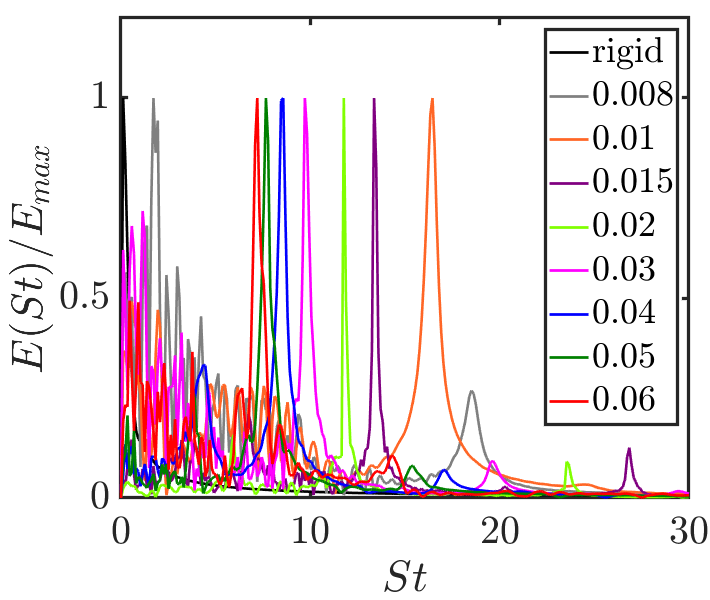
\includegraphics[width=1\linewidth]{Figures/FlowFrequency/Freq_Mode.png}
		\end{minipage} 
		\begin{minipage}[c]{0.485\linewidth}
			\begin{overpic}[width=1\linewidth]{Figures/FlowFrequency/Freq_Ca.png}
				\put(-215,200){{\parbox{1\linewidth}{$(a)$}}}	
				\put(-4,200){{\parbox{1\linewidth}{$(b)$}}}	
				\put(46,88){{\parbox{1\linewidth}{\rotatebox{87}{$transiton$}}}}
			\end{overpic}
		\end{minipage} 
		\caption{(a) Frequency energy spectra of streamwise velocity probed at slit exit next to the plate (2.2h,0.5h) is shown. The energy axis is normalized by its self maximum value. (b) Dominant frequency for the different flexible plate case, $Ca$. The cross mark in the inset figure marks the position (2.2h,0.5h).}
		\label{fig:flow_fft_S_3D}
	\end{figure}

During the periodic jetting phenomenon, the most prominent vortex structure, i.e., the leading vortex structure (LVP), detaches and propagates through the channel. The detached LVP speeds up through the channel. 
Figure \ref{fig:vortPnC}(a) shows the propagation rate for different cases of $Ca$. The black curve represents the downstream channel propagation of the leading vortex pair for the rigid plate case. With an increase in the plates' flexibility, the vortex gains a sudden release of energy as the vortex sheds off the tip of the oscillating plate. This throw increases the rate of propagation higher than that in the rigid plate case. With increasing $Ca$, the starting velocity of the leading vortex pair is shown in Figure \ref{fig:vortPnC}(b). Interestingly, the resulting trend is non-monotonic for the given range of $Ca$. The LVP attains its highest starting velocity at the case with $Ca=0.03$ and reduces thereafter for more flexible cases. This is because cases with even more flexibility begin to cause more agitation into the flow, such as backflow and interactions among the vortex pairs themselves.


In Figure \ref{fig:vort_evo_1S_4S}, we show a one-to-one comparison of the development of vortical structures in the flow over time for the rigid and flexible plate ($Ca=0.02$) case. In the top panel $(a-d)$, we sequentially see the vortices shearing off the tip of each rigid plate. The vortices are shown in red as anti-clockwise flow movements and blue as clockwise. These bloom up over time and are continuously being fed to grow larger in a self-similar fashion. In contrast, the bottom panels $(e-f)$ in the figure are for a flexible plate case ($Ca=0.02$). The flexible plates, under the effect of inlet flow inertia, bend with the stream, and the flow shears over the flexible plate from the fixed end to the free end. This sudden bend causes a throwback of the flow off the plates' tip in the upstream direction (panel $(e)$) in the form of vortical structures as long as the plate moves in the downstream direction. These back vortices grow gradually for a short duration but subsequently get suppressed due to the flow inertia. Now, as the flexible plate attains backward motion in the oscillation, the tip edges generate a vortex in the downstream direction (panel $(f)$). This generated vortex grows as long as the next oscillation cycle of the plates kicks in, which causes the change of direction in the plates' motion. This sudden reversed motion cuts-off the vorticity being fed into the vortex pair and thus dissociates off the plates' edges (panel $(g)$). This vortex pair gathers vorticity and propels further into the downstream due to its self-propagating nature. This phenomenon is called as "pinch-off" of the vortex pair, which is found absent in the rigid plate case. It can be understood that a new time-scale in terms of flexible plate oscillations is involved in the phenomena, unlike the convective time-scale as in the rigid plate case. Panel $(h)$ shows the generation of subsequent vortex pair as the next oscillation cycles prevail.

	\begin{figure}[h]
	\centering
	\begin{minipage}[c]{0.48\linewidth}
		\centering
		\begin{overpic}[width=1\linewidth]{Figures/timespace/time-space_S2p1.png} 			\put(-5,165){{\parbox{1\linewidth}{$(a)$}}}	
			\put(130,35){{\parbox{1\linewidth}{$Ca=0.001$}}}	
		\end{overpic}
	\end{minipage}
	\begin{minipage}[c]{0.48\linewidth}
		\centering
		\begin{overpic}[width=1\linewidth]{Figures/timespace/time-space_S3p1.png} 				\put(-5,165){{\parbox{1\linewidth}{$(b)$}}}	
			\put(135,35){{\parbox{1\linewidth}{$Ca=0.01$}}}	
		\end{overpic}
	\end{minipage}
	\begin{minipage}[c]{0.48\linewidth}
		\centering
		\begin{overpic}[width=1\linewidth]{Figures/timespace/time-space_S4.png} 				\put(-5,165){{\parbox{1\linewidth}{$(c)$}}}	
			\put(135,35){{\parbox{1\linewidth}{$Ca=0.02$}}}	
		\end{overpic}
	\end{minipage}
	\begin{minipage}[c]{0.48\linewidth}
		\centering
		\begin{overpic}[width=1\linewidth]{Figures/timespace/time-space_S5.png} 				\put(-5,165){{\parbox{1\linewidth}{$(d)$}}}	
			\put(135,35){{\parbox{1\linewidth}{$Ca=0.04$}}}	
		\end{overpic}
	\end{minipage}
	\caption{(a) Normalized circulation of the leading vortex pair (LVP) over time. (b) Circulation within the LVP for flexible plate case in comparison to the rigid plate case.}
	\label{fig:time_space_all}
\end{figure}

It is evident from the study that steady inlet flow can be triggered to generate periodic train of vortex pair by the use of flexible plates. To analyse the shedding frequency of the these vortex pairs off the plates oscillating motion, we investigate the stream-wise velocity at a point immediately next to the slit opening ($(2.2h,0.5h)$ as a probe (see the cross mark in the inset figure of Fig~\ref{fig:flow_fft_S_3D}(b)). %The flexible plates induce more oscillations and fluctuations in the fluid system; thus, transverse velocities increase at the cost of stream-wise inertia.
Figure \ref{fig:flow_fft_S_3D}(a), show an FFT analysis for the time signal of the probed streamwise velocity. The plot shows normalised energy spectra for the involved non-dimensional frequencies ($St_f=fh/u_{o}$, where $f$ is the streamwise flow frequency) in the time signal. In panel $b$, the dominant frequency is shown for the range of $Ca$ cases studied. We see a critical value of $St \approx 16$ at $Ca=0.01$ which marks transition from steady jet flow to pulsed oscillation of the flow in the form of periodic vortex pairs. This jump resembles similar to the classical supercritical Hopf bifurcation. Such a transformation suggests a neat periodic pumping of the steady flow. In our cases, the flexible plates act like periodic catapults which store and release energy to induce periodicity in the flow. This suggests that the leading vortex pair pinch-off is linked with the backstroke of the plates' oscillation. As the plates' oscillation period reduces (with increasing $Ca$), the vortex pair pinch-off rate also reduces. This is a crucial result that highlights the effect of time-scale associated with flexible plate oscillations over the convective time-scale on the vortex pair pinch-off.

To have an overview on the flow breakup pattern over time in the form of vortical ejections through the slit we show time-space distribution of the vertically integrated vorticity in figure \ref{fig:time_space_all}. Four different cases with $(a)\ Ca=0.001$, $(b)\ Ca=0.01$, $(c)\ Ca=0.02$, and $(d)\ Ca=0.04$ are shown in the figure. As discussed previously, the fringe pattern shows the presence of multiple vortex structures in the flow. For $Ca=0.001$, the LVP stays connected for a while before it gets unstable and further roll ups of the incoming vortices can be seen as the fringes in time-space map. In case of more flexible plate case, $Ca=0.01$ the subsequent vortices generate at early times in periodic fashion as the pinch-off phenomena is observed in the flow. Similarily, transition of steady inlet flow through the slits to periodic outflow into the downstream can be observed in even higher $Ca$ cases. In figure \ref{fig:time_space_all}(d), it is worth to notice a gap between initial trace and rest of the fringed pattern. This attributes to the higher velocity attained by the leading vortex pair in $Ca=0.04$ case because of which it leads ahead than rest of the periodic flow.



\section{Summary}\label{sec:Summary}

This work investigated the starting flow through a narrow slit gap, both with rigid and flexible plates. Our comprehensive study on the leading vortex pair (LVP) formation, growth, and propagation showed a key insight into how the LVP behaves in a confined and unbounded environment and how the rigid and flexible nature of the plate alters the LVP's behavior. It has been found that the vortex pair pinch-off and periodic generation of vortex pairs can be induced with flexible plates, a phenomenon absent in the rigid plate case.

The study investigated into the physics of fluid flow within a confined two-dimensional channel, specifically probing the fluid dynamics emerging in the vicinity of wall-mounted flexible plates. The channel design involved dimensions dictated by a height parameter ($h$), with two plates positioned opposite each other at a distance ($2h$) from the inlet. The plates, characterized by a length of $0.425h$, were engineered to have varying flexibility, represented by the Cauchy Number ($Ca$). At the channel's inlet, a fully developed parabolic flow was established, setting the stage for a laminar flow pattern with a predetermined Reynolds number ($Re_\infty$) of $500$. This inlet profile and the configuration led to intricate flow structures, most notably the "mushroom"-like structure termed as the 'leading vortex pair' (LVP). The LVP's formation is induced by the acceleration of fluid as it navigates through the narrow slit formed between the plates. The subsequent downstream movement of the LVP is accompanied by a trailing shear layer connected to the slit edges. The LVP and its trailing shear layer manifest intriguing dynamics, influenced by the channel walls which govern their growth and movement. To gain a deeper understanding, a comparative analysis was also conducted between the main setup ("bounded" case) and a counterpart with wider channel openings ("unbounded" case). This comparison revealed the constraining effects of the channel walls on the flow dynamics, especially on the growth of fluid structures. Fluid flow in a confined channel in the presence of wall-mounted flexible plates, showcases intricate and complex dynamics. The study highlighted the importance of understanding such interactions, especially when designing systems that involve fluid-structure interactions. This understanding opens the opportunity for designing efficient and controlled fluid transport systems, where the leading vortex pair can be manipulated by varying the plate flexibility. This can help in the design of efficient fluidic devices where the vortex pair's behavior can significantly impact the fluid flow and transport.

One of the most prominent outcomes of the flow dynamics is the formation of the 'leading vortex pair' (LVP). This mushroom-like structure, resulting from the fluid's acceleration through the slit, serves as a testament to the intricacies involved in confined fluid dynamics. The impact of channel walls on flow dynamics was evident. The "bounded" case, where flow was restricted by the channel walls, showed a more contained growth of the LVP and its trailing shear layer compared to the expansive growth observed in the "unbounded" case. The flexibility of the plates, represented by the Cauchy Number $Ca$, was pivotal in dictating the nature of the fluid-plate interactions. This parameter can be seen as a vital tool for modulating flow behavior in confined spaces. While the study shed light on various facets of the fluid dynamics in confined spaces, the eventual destabilization of the LVP downstream prompts further investigation. A deeper dive into the mathematical modelling for the correlation between structural behaviour and corresponding destabilization of the LVP can serve as a crucial scope for future research in this domain. 
In summation, the present study reinforces the significance of understanding fluid dynamics in confined spaces, especially when coupled with flexible structural elements. Such insights are vital in designing efficient fluid-transport systems and deciphering similar natural phenomena.



\section*{Ackowledgments}
	We thank the fellow members of Computational Mechanics Group, IIT Kharagpur, for their support. We acknowledge research grants from the Board of Research and Nuclear Science(BRNS) and the Mathematical Research Impact Centric Support (MATRICS) scheme sponsored by the Government of India to study multiphase flow. We sincerely thank Param Shakti for computing resources developed under National Supercomputing Mission at IIT Kharagpur, India.

\bibliographystyle{elsarticle-harv} 
\bibliography{pre2}

%% else use the following coding to input the bibitems directly in the
%% TeX file.

% \begin{thebibliography}{00}

% %% \bibitem[Author(year)]{label}
% %% Text of bibliographic item

% \bibitem[ ()]{}

% \end{thebibliography}
\end{document}

\endinput
%%
%% End of file `elsarticle-template-harv.tex'.
